\addcontentsline{toc}{section}{Введение}
\chapter{Введение}
\justify
Проблема поиска пересечений линий на изображении является очень распространенной и её решение может быть использовано в таких задачах компьютерного зрения как:
\begin{enumerate}
	\item Автоматическое определение полей во время спортивных трансляций
	\item Детектирование ориентиров при автоматическом управлении роботом
	\item Детектирование железнодорожных стрелок на изображении, сделанном с локомотива поезда
\end{enumerate} 

Для автоматизации процесса управления поездом необходимо создать систему, которая позволяла бы стать надежным автоматическим ассистентом/помощником для машиниста локомотива (стать неким driving assistance), но ни в коем случае не заменить действия человека полностью. 
Одной из задач такой системы является обнаружение железнодорожных стрелок для обеспечения движения поезда по правильному пути.
Решение этой задачи позволит обнаруживать разветвления пути заранее (визуально) и анализировать возможные дальнейшие пути движения поезда, выдавая полезную информацию для машиниста локомотива, такую как: "на правой ветке обнаружены вагоны - путь занят!". Это решение значительно повысит безопасность движения на железных дорогах.

\textbf{Целью данной работы} является разработка алгоритма детектирования железнодорожных стрелок на изображении, сделанном с локомотива поезда. Таким образом, необходимо решить следующие задачи:
\begin{enumerate}
	\item Разметить датасет из ж/д стрелок на изображениях, сделанных с локомотива поезда.
	\item Разработать алгоритм поиска стрелок на основе преобразования Хафа\cite{b:hough_transform} и геометрических особенностей различных видов ж/д стрелок.
	\item Обучить SVM\cite{b:SVM}-классификатор, который по входной гистограмме ориентированных градиентов\cite{b:HOG} смог бы предсказать - cоответствует эта гистограмма изображению железнодорожной стрелки или нет.
	\item Привести результаты работы обоих алгоритмов на размеченном датасете и сравнить алгоритмы.
\end{enumerate}


\newpage
\section{Постановка задачи}
На вход подается изображение — фотография сделанная с головы поезда. Необходимо найти на входном изображении места пересечений железно-дорожных путей. Пересечением будем называть точку, в которой пересекаются рельсы одной ж/д колеи с другой. На выходе алгоритма должен быть набор точек, в которых было обнаружено пересечение.

\begin{figure}[!h]
	\centering
	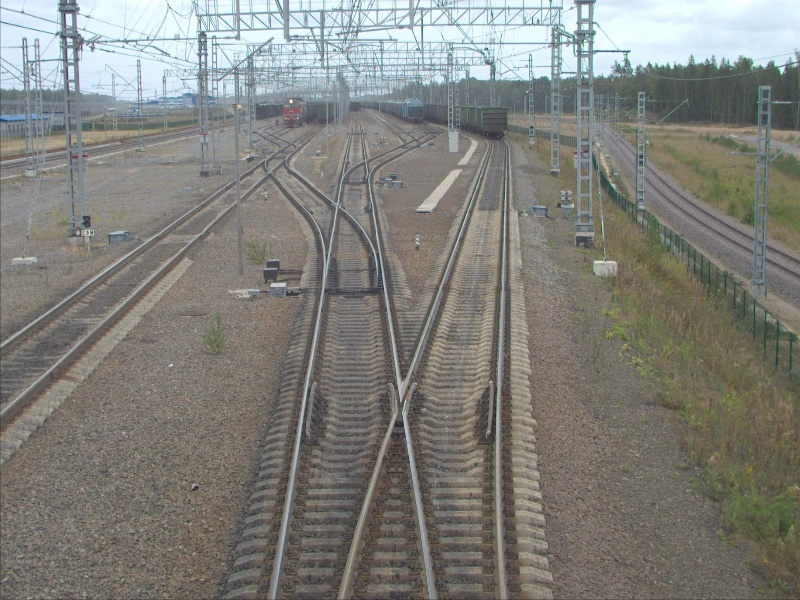
\includegraphics[width=0.9\textwidth]{pictures/img0002.jpg} 
	\caption{Пример входного изображения}
	\label{fig:input}
\end{figure}

\newpage
Замечания: 
\begin{enumerate}
	\item Точность поиска стрелок - окрестность от 20x20 до 50x50 пикселей(в зависимости от дальности стрелки)
	\item Необходимо правильно находить стрелки в пределах 20-30 метрах перед поездом. Нет задачи детектировать стрелки, которые находятся слишком далеко от поезда(40 метров и далее).
\end{enumerate}

\section{Обзор литературы}
\label{obzor}
Существует несколько глобальных подходов к поиску объектов на изображении:
\begin{enumerate}
	\item Сопоставление границ, градиентов и чёрно-белых пикселей изображения. Этот подход устойчив к изменению света, но не устойчив к изменению положения объекта на изображении(вращение, угол наклона).\cite{b:edge_match}.
	\item Поиск объекта по геометрическим свойствам. Если форма искомого объекта может быть задача аналитически, то такие объекты можно искать с помощью преобразования Хафа \cite{b:hough_transform}.
	\item Подход, основанный на сопоставлении признаков ключевых точек изображения с ключевыми точками искомого объекта. Данный подход реализован в следующих методах: SIFT\cite{b:SIFT}, SURF\cite{b:SURF}.
	\item Обучение классификатора на размеченных данных. В роли классификатора может быть: SVM классификатор\cite{b:SVM}, дерево решений \cite{b:decision_tree}, KNN классификатор \cite{b:knn}. В качестве входных векторов для классификаторов могут быть использованы различные виды признаков, полученные из размеченных изображений. 
	Например, гистограмма ориентированных градиентов(HOG)\cite{b:HOG},
	SURF\cite{b:SIFT}/SIFT\cite{b:SURF} дескрипторы и так далее. 
\end{enumerate}
Рассмотрим данные подходы подробнее.
\subsection{Поиск объекта по его геометрическим свойствам}
Для поиска объектов, геометрическая форма которых может быть задана некоторым уравнением(н-р прямая, круг, эллипс) используется следующий подход:
\begin{enumerate}
	\item Из изображения извлекаются границы. Это можно сделать с помощью алгоритма Canny \cite{b:canny}. \newline
	Пример применения алгоритма Canny к входному изображению:
	\begin{figure}[!h]
		\centering
		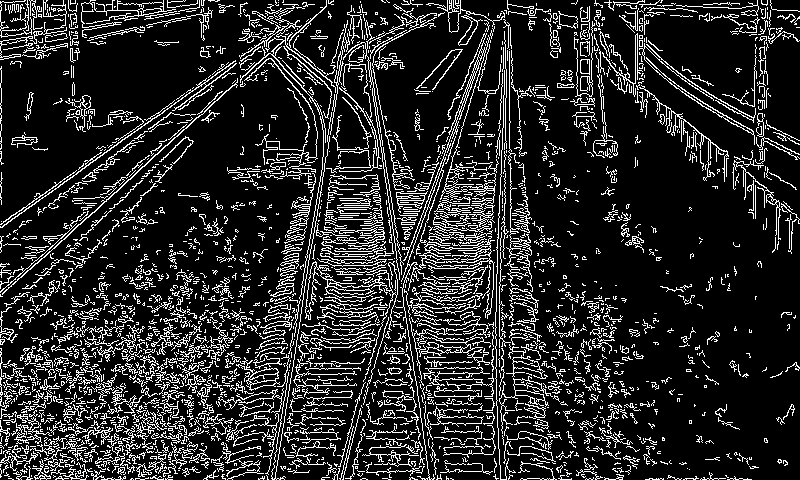
\includegraphics[width=0.9\textwidth]{pictures/canny_res.png}
		\caption[Применение алгоритма Canny]{Алгоритм Canny}
		\label{fig:cannyres}
	\end{figure}
	\item После чего к полученным границам применяется алгоритма Хафа \cite{b:hough_transform}. Если целью является поиск прямых, то алгоритм Хафа даст следующий результат(красным обозначены найденные линии):
	\begin{figure}[!h]
		\centering
		\begin{minipage}{0.45\textwidth}
			\centering
			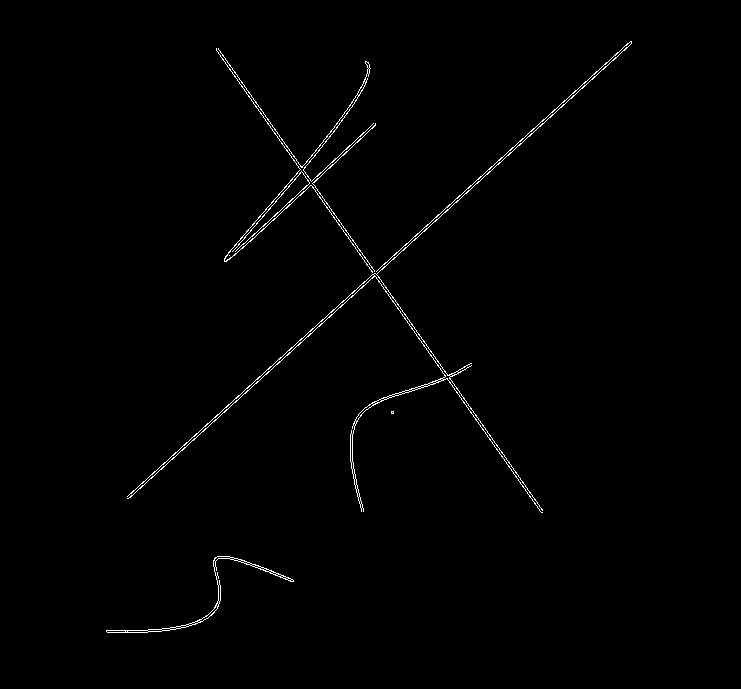
\includegraphics[width=0.7\linewidth]{pictures/canny_ex}
			\caption[Y]{Алгоритма Canny}
			\label{fig:canny_ex}
		\end{minipage}
		\begin{minipage}{0.45\textwidth}
			\centering
			
\includegraphics[width=0.7\linewidth]{pictures/hough_ex}
			\caption[X]{Поиск прямых}
			\label{fig:hough_ex}
		\end{minipage}
	\end{figure}
\end{enumerate}

Таким образом, если требуется искать пересечения прямых линий на изображении, то для этого отлично подойдет следующий алгоритм:
\begin{enumerate}
	\item Поиск границ \cite{b:canny}
	\item Поиск линий \cite{b:hough_transform}
	\item Поиск пересечений линий, найденных в предыдущем шаге. Это можно сделать аналитически. Для каждой пары найденных прямых составляем систему уравнений, тогда если эти прямые не параллельны, то решением системы будет точка пересечения прямых.
	$
	\begin{cases}
	a_1x + b_1y = c_1 
	\\
	a_2x + b_2y = c_2 
	\end{cases}
	$
\end{enumerate}

\paragraph{Предыдущие работы, посвященные поиску ж/д путей и их пересечений с помощью применения геометрически ориентированного подхода}

\subparagraph{Vision based rail track and switch recognition for self-localization of trains in a rail network \cite{b:hough_work1}.}

Подход, описанный в данной работе основан на анализе изображения с камеры, стоящей в голове
поезда. Условиями для корректного определения стрелок на железной дороге является то, что
расстояние между параллельными рельсами всегда одинаковое, а также радиус кривизны рельсов
достаточно большой.

В данной работе съёмка ж/д путей происходит достаточно часто, и к каждому вновь сделанному снимку применяется следующий алгоритм:

1. Из изображения вырезается близкая к поезду полоса.
\begin{figure}[!h]
	\centering
	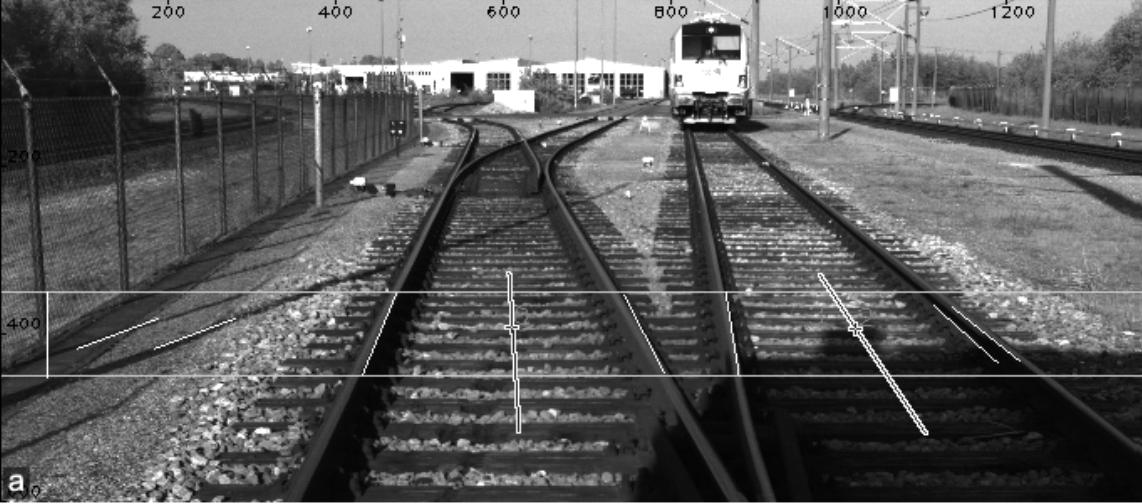
\includegraphics[width=0.9\linewidth]{pictures/screenshot001}
	\caption{Горизонтальный блок}
	\label{fig:screenshot001}
\end{figure}

2. К выделенному участку применяется алгоритм поиска ребер: 
\begin{enumerate}
	\item Рассчитывается вектор градиента в каждой точке изображения
	\item Далее рассматриваются окрестности по 3x3 пикселя. И для каждого пикселя с величиной градиента большей, чем у половины соседей в окрестности выполняется следующая
	процедура: 
	Строится матрица ковариаций данного пикселя с соседями в окрестности 3х3. 
	$
	S = \left(
	\begin{array}{cccc}
	Cov_{xx} & Cov_{xy}\\
	Cov_{yx} & Cov_{yy}\\
	\end{array}
	\right), где
	Cov_{ab} = \dfrac{1}{N} \sum_{1}^{N} (g_a, g_b)
	$, так как среднее значение градиента для черно-белого изображения равняется нулю. 
	\item Вычисляются собственные числа этой матрицы, и если выполнены неравенства:
	$
	\begin{cases}
	\lambda_1 \geq t_l\\
	\dfrac{\lambda_2}{\lambda_1} \geq m_l 
	\end{cases}
	$
	,где $t_l, m_l$ вычисленные эмперическим путём константы, то данный пиксель считается
	краевым.
	Также из матрицы ковариации получаются два собственных вектора:
	$e_1, e_2$, больший из которые перпендикулярен краю, а меньший параллелен краю в данной точке.
\end{enumerate}
В итоге границы найденные границы выделенного блока выглядят следующим образом:
\begin{figure}[!h]
	\centering
	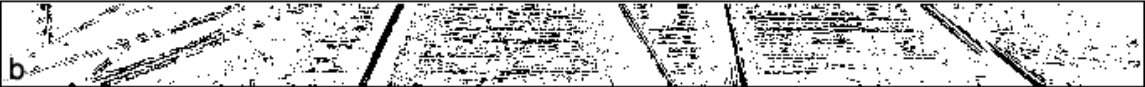
\includegraphics[width=0.9\linewidth]{pictures/screenshot002}
	\caption{Границы в блоке}
	\label{fig:screenshot002}
\end{figure}

3. Поиск прямых.

Строится массив аккумулятор$A(\theta, x)$(по аналогии с алгоритмом Хафа\cite{b:hough_transform}). И для каждого краевого пикселя(K) вычисляется угол $\theta$ между большим собственным вектором $e_2$ и осью OY. 
Также необходимо вычислить значение $x_c$. Строится дополнительная прямая $y_c$ = $\dfrac{H}{2}$, где H - высота рассматриваемого изображения. Тогда $x_c$ будет координатой $x$ точки пересечения построенной прямой $y_c$ и продолжения собственного вектора $e_2$.
Увеличиваем значения аккумулятора $A(\theta, x_c)$ = $A(\theta, x_c) + 1$.
В итоге максимумы аккумулятора будут соответствовать параметрам прямых линий на изображении. На рисунке найденные линии обозначены черными точками.
\begin{figure}[!h]
	\centering
	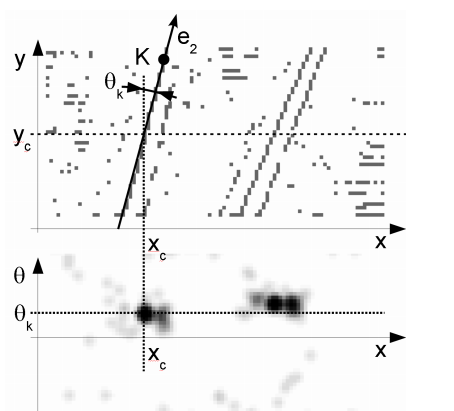
\includegraphics[width=0.5\linewidth]{pictures/screenshot004}
	\caption{Поиск линий}
	\label{fig:screenshot004}
\end{figure}
\newpage
Данный алгоритм работает значительно быстрее преобразования Хафа(ускорение достигается за счет сохранения времени, которое в алгоритме Хафа тратится на перебор $\theta \in [0, \pi]$). Угол $\theta$ в каждой краевой точке высчитывается с помощью направления собственного вектора матрицы ковариаций в данной точке($\theta$= $\angle(e_2, OY)$). 
При этом алгоритм качественно находит прямые линии, проходящие через центральную вертикальную ось изображения.

Существуют и другие алгоритмы, позволяющие ускорить оригинальный алгоритм Хафа. Например \cite{b:hough_fast}.
4. Выделение ж/д колеи по найденным прямым.

В данном алгоритме предполагается, что ширина железнодорожной колеи заранее зафиксирована и приходит на вход алгоритму. 

Поэтому чтобы найти пары рельсов, принадлежащих к одной колее нужно выполнить перебор по всем найденным рельсам, сравнивая при этом расстояние между ними с эталонным расстоянием между рельсами(с некоторой погрешностью $\delta R$).

Но нельзя забывать про то, что изображение делается с камеры и нужно учитывать перспективную проекцию \cite{b:projection} точек изображения на точки в реальном мире, чтобы корректно сравнивать расстояние между рельсами на изображении с расстоянием в мировой системе координат. 
В итоге результат поиска ж/д колеи следующий(на рисунке выделен горизонтальный блок и линии, соответствующие центрам найденных пар рельсов):
\begin{figure}[!h]
	\centering
	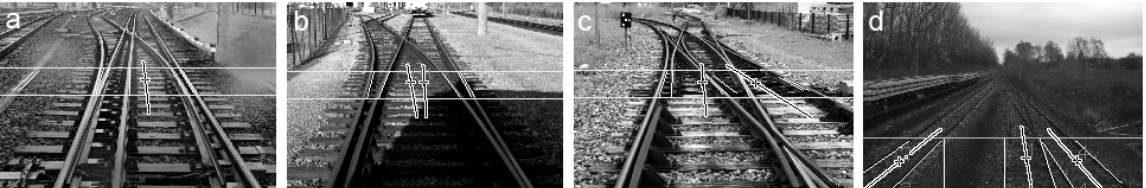
\includegraphics[width=1\linewidth,height=0.5\linewidth]{pictures/screenshot006}
	\caption{Центр колеи}
	\label{fig:screenshot006}
\end{figure}

5. Определение стрелок.

При поиске пересечений найденных рельсов учтем, что нам известен минимальный радиус
кривой, по которой может двигаться поезд(является параметром алгоритма). Из данного радиуса можно вычислить максимальное боковое отклонение $s_1$, на которое должен отклониться центр колеи, чтобы считаться пройденной колеёй. 

Таким образом, мы ожидаем, что одна из наблюдаемых нами колея всегда имеет боковое отклонение от центра поезда принадлежащее интервалу [$-s_1$, $s_1$].
Если центр колеи становится < $-s_1$, то это означается, что данная колея является левой веткой колеи, по которой поезд движется в данный момент времени. В обратном случае правой веткой. В момент времени, когда происходит переход данной границы мы можем отметить, что поезд прошел стрелку.
На рисунке\ref{fig:screenshot008} обозначены границы $s_1$(теоретическая граница) и $s_2$(экспериментальная граница), где $s_2$ = $s_1$ + $\delta s$(подобрана экспериментально). Пересечение фиксируется в момент времени, когда центр колеи переходит границу $|s_2|$(это место показано стрелками на рисунке).
\begin{figure}[!h]
	\centering
	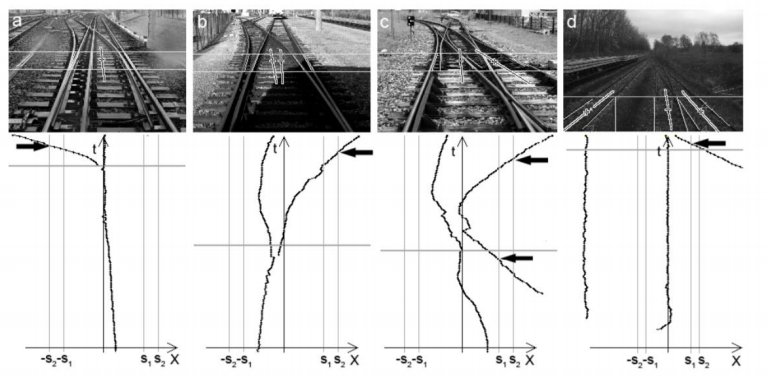
\includegraphics[width=1\linewidth]{pictures/screenshot008}
	\caption{Перемещение X центра колеи}
	\label{fig:screenshot008}
\end{figure}

На втором слева рисунке видно, что сначала есть отметка только от колеи, идущей прямо. Потом появляется отметка от колеи отклоняющейся налево. После появления отклоняющейся колеи, отметка от прямой колеи отклоняется направо, а отметка от отклоняющейся колеи остается в центре - следовательно поезд пошёл по отклоняющейся колее, так как теперь её координата центра находится ближе всего к середине поезда. В момент, когда отметка от центра прямого пути проходит порог $s_2$ отмечается стрелка.

На последнем рисунке сначала есть отметка от двух параллельных путей. Потом появляется отметка от присоединяющегося справа пути. И в момент, когда координата центра присоединяющегося пути проходит порог $s_1$ отмечается стрелка.

\subparagraph{Efficient railway tracks detection and turnouts recognition method using HOG features \cite{b:growing_up}}.
\label{growing_up}

В данном работе описывается метод поиска железнодорожных путей с использованием Histogram of oriented gradients\cite{b:HOG}(гистограмма ориентированных градиентов).

Алгоритм следующий:
1. Входное изображение разбивается на сетку, с уменьшением размера блока в зависимости от координаты Y на изображении(это сделано чтобы имитировать перспективную проекцию).
\begin{figure}[!h]
	\centering
	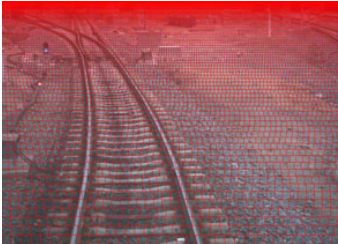
\includegraphics[width=0.5\linewidth]{pictures/screenshot009}
	\caption{Разбиение на сетку}
	\label{fig:screenshot009}
\end{figure}

2. Начиная с нижней строки сетки применяется алгоритм growing up, который на основе похожести HOG соседних верхних клеток расширяет множество схожих кусочкой изображения.
В итоге на выходе алгоритма growing up имеем множество рельсов(на рисунке обозначены разными цветами).
\begin{figure}[!h]
	\centering
	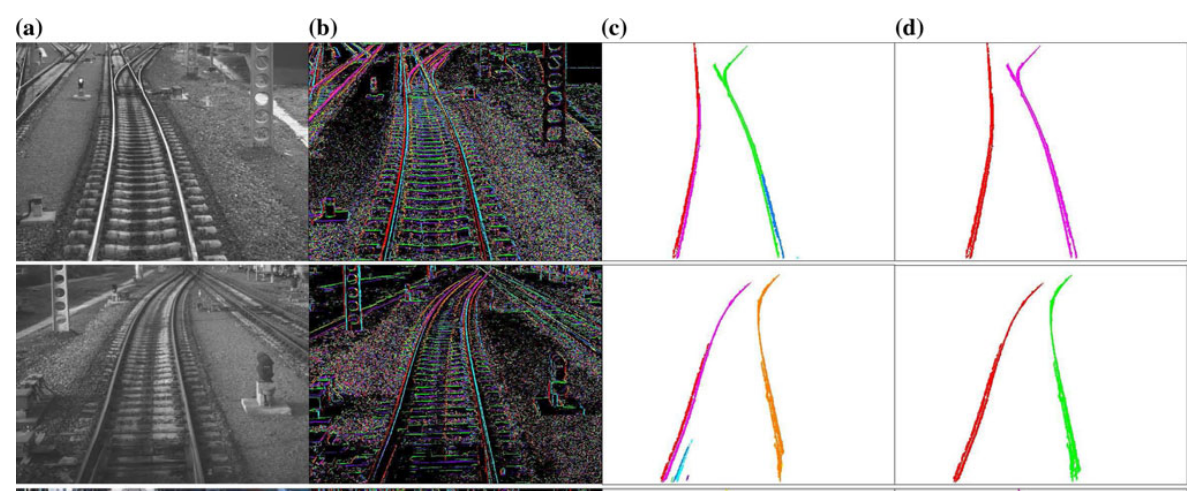
\includegraphics[width=1\linewidth]{pictures/screenshot010}
	\caption{Результат поиска рельсов}
	\label{fig:screenshot010}
\end{figure}
\newpage
\paragraph{Поиск полосы движения автомобиля \cite{b:lane_detection}}.
Для решения задачи поиска стрелок полезно уметь находить сами ж/д пути.
Задача поиска ж/д пути тесно связана с задачей поиска полосы движения автомобиля(lane detection). Рассмотрим несколько работ, посвященных этой теме.

\subparagraph{Robust lane detection and tracking for lane departure warning}
В работе \cite{b:lane_detection} предложен следующий алгоритм для поиска полосы движения автомобиля:

Поиск границ на изображении с помощью алгоритма Canny \ref{fig:screenshot00232}(b).
После чего удаляются все горизонтальные линии \ref{fig:screenshot00232}(c). И далее удаляются одиночные пиксели, которые тоже являются шумом \ref{fig:screenshot00232}(d).
\begin{figure}[!h]
	\centering
	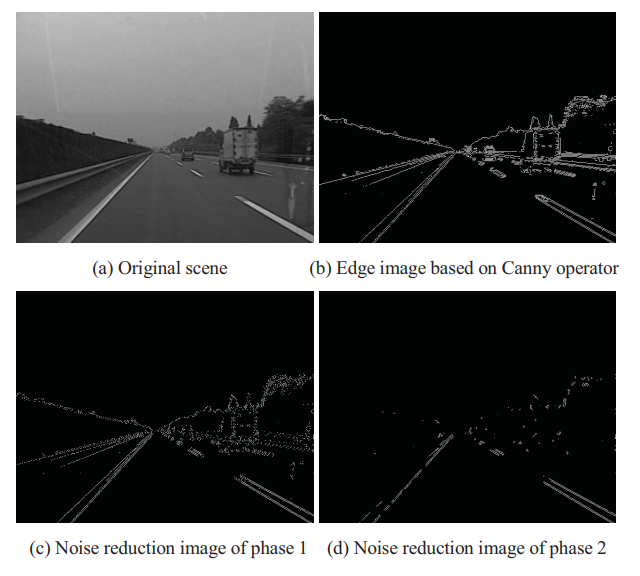
\includegraphics[width=0.5\linewidth]{pictures/screenshot00232}
	\caption{Избавление от шума}
	\label{fig:screenshot00232}
\end{figure}
\newpage

Далее рассматривается нижняя четверть полученного изображения. И проводится "сканирующая линия", на которой считаются интенсивности пикселей и строится график интенсивности в зависимости от горизонтально позиции пикселя на линии \ref{fig:screenshot00233}(b).
\begin{figure}[h!]
	\centering
	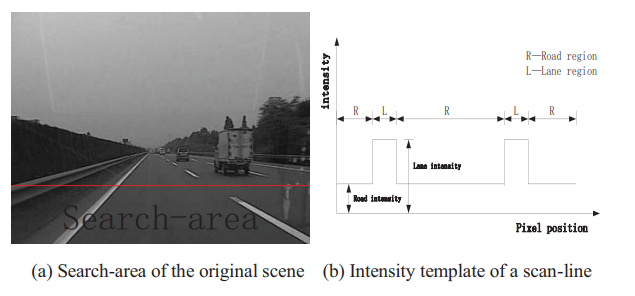
\includegraphics[width=1\linewidth]{pictures/screenshot00233}
	\caption{График интенсивности}
	\label{fig:screenshot00233}
\end{figure}

Видно, что интенсивность в районе разметки сильно изменяется относительно дороги. Применяя такую процедуру на каждом кадре можно детектировать полосу в непосредственной близости перед автомобилем. Итоговый результат детектирования полосы:
\begin{figure}[!h]
	\centering
	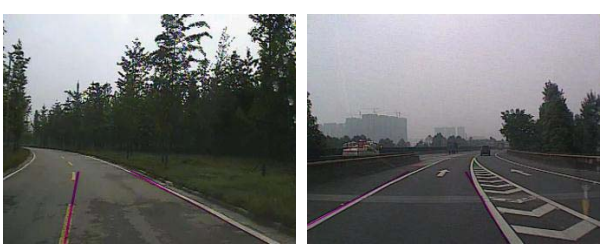
\includegraphics[width=1\linewidth]{pictures/screenshot00234}
	\caption{Результат поиска полосы}
	\label{fig:screenshot00234}
\end{figure}

\subparagraph{Double Lane Line Edge Detection Method Based on Constraint Conditions Hough Transform}
В работе \cite{b:lane_detection_hough} предложен алгоритм на основе преобразования Хафа\cite{b:hough_transform}:
Сначала учитывается то, что R и G компоненты цвета для полосы движения значительно выше, чем у самой дорого(высокие значение R и G говорят о желтом оттенке). В связи с этим цвета пикселей изображения преобразуются для удаления лишних шумов:
\begin{figure}[!h]
	\centering
	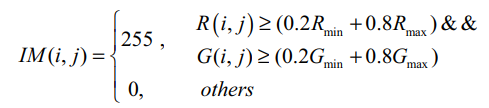
\includegraphics[width=0.7\linewidth]{pictures/screenshot025}
	\caption{}
	\label{fig:screenshot025}
\end{figure}

После чего изображение разделяется на три горизонтальный блока: близкий, средний и дальний.
\begin{figure}[!h]
	\centering
	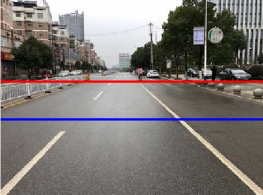
\includegraphics[width=0.7\linewidth,height=0.4\linewidth]{pictures/screenshot026}
	\caption{Разделение на блоки}
	\label{fig:screenshot026}
\end{figure}
\newpage
Далее применяется алгоритм Canny\cite{b:canny} для поиска границ. И ищутся прямые линии с помощью преобразования Хафа \cite{b:hough_transform}.
\begin{figure}[h!]
	\centering
	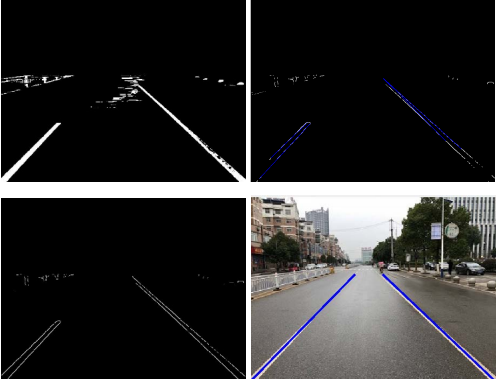
\includegraphics[width=0.7\linewidth]{pictures/screenshot027}
	\caption{Применение алгоритма Хафа}
	\label{fig:screenshot027}
\end{figure}

В случае, когда дорога имеет поворот применяется следующая процедура. Считается, что поворот можно описать параболической линией. Поэтому в ближней части прямые ищутся, как и прежде, через преобразование Хафа \cite{b:hough_transform}, а в средней части как парабола($y_m$ - координата прямой разделяющей ближнюю и среднюю части изображения, a и b - параметры прямой):

$x = a + by + cy^2$ - уравнение параболы

$
x =  
\begin{cases}
a + by, y \le y_m 
\\
c + dy + ey^2, y > y_m 
\end{cases}
$

Теперь для средней зоны ищется продолжение найденных в ближней зоны прямых.
Это делается просто проходом с разными шагами по координате Х и поиска последовательности точек, которая удовлетворяла бы уравнению параболы. В итоге результат получается следующий:
\begin{figure}[h!]
	\centering
	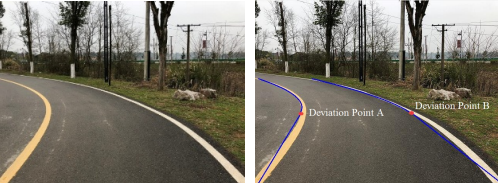
\includegraphics[width=1\linewidth]{pictures/screenshot029}
	\caption{Результат поиска дороги}
	\label{fig:screenshot029}
\end{figure}

\subparagraph{A New Lane Line Segmentation and Detection Method based on Inverse Perspective Mapping\cite{b:inverse_mapping}}
В данной работе описан подход для поиска полосы движения автомобиля, основанный на технике "Inverse Mapping". Точки проецируется из 2D картинки на 3D объект с помощью закона перспективного проецирования\cite{b:projection}, после чего точка 3D объекта проецируется ещё раз на 2D плоскость таким образом, чтобы избежать эффекта перспективы на 2D изображении. В итоге получается следующий результат:
\begin{figure}[h!]
	\centering
	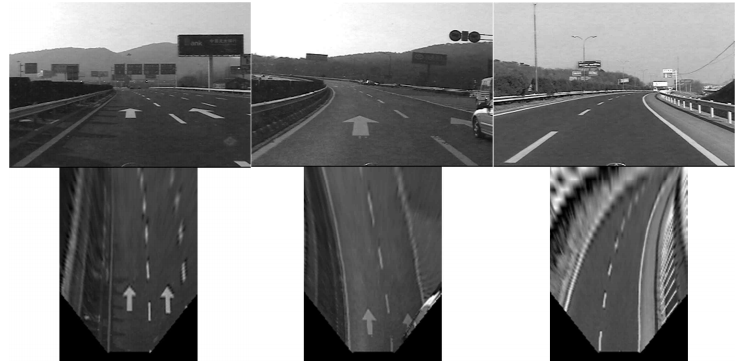
\includegraphics[width=0.7\linewidth]{pictures/screenshot23234}
	\caption{Inverse Perspective Mapping}
	\label{fig:screenshot23234}
\end{figure}

После чего на полученном изображении параллельные прямые, соответствующие линиям разметки, становятся действительно близкими к параллельным и можно применить алгоритма Хафа для поиска прямых\cite{b:hough_transform} и получить следующий результат детектирования полосы движения:
\begin{figure}[h!]
	\centering
	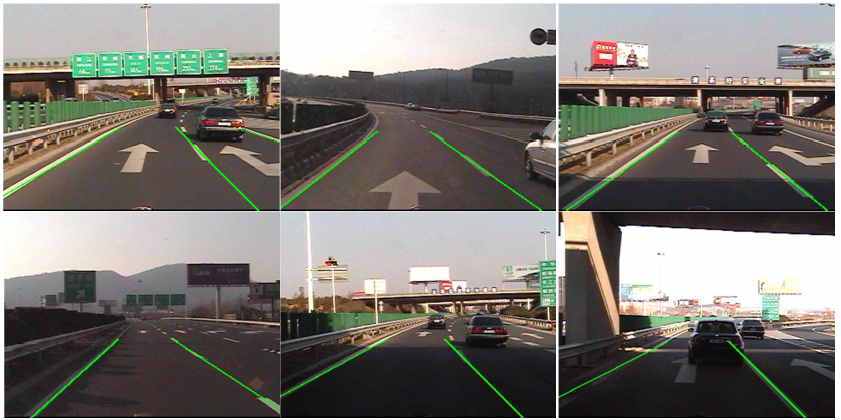
\includegraphics[width=0.7\linewidth]{pictures/screenshot23235}
	\caption[Результат детектирования полосы]{Результат детектирования полосы}
	\label{fig:screenshot23235}
\end{figure}

Технику "Inverse Mapping" можно применять и для задачи поиска стрелок на изображении. Действительно, если сделать "Inverse Mapping" изображения, сделанного с локомотива поезда можно было бы получить  изображение без эффекта перспективы и на нём прямые линии будет найти проще, чем на исходном изображении. Однако, в нашей задаче параметры камеры, которая установлена на локомотиве неизвестные, поэтому сделать правильный "Inverse Mapping" не удастся, что будет приводить к непредсказуемому итоговому результату.

%	\label{fig:screenshot23231}
\newpage
\subsection{Поиск объекта по ключевым точкам}
Одним из методов поиска объектов на изображении является построение SIFT\cite{b:SIFT} дескриптора и сопоставление этого дескриптора с SIFT дескриптором искомого объекта.

Сначала изображение преобразуется в большой набор векторов признаков(SIFT дескриптор), каждый из которых инвариантен относительно параллельного переноса изображения, масштабирования и вращения, частично инвариантен изменению освещения и устойчив к локальным геометрическим искажениям.

После чего SIFT дескриптор текущего изображения и искомого объекта сопоставляются и на выходе можно увидеть соответствие ключевых точек на изображении и ключевых точек искомого объекта:
\begin{figure}[!h]
	\centering
	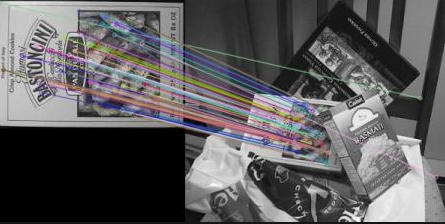
\includegraphics[width=1\linewidth]{pictures/screenshot011}
	\caption{SIFT пример}
	\label{fig:screenshot011}
\end{figure}

Если говорить о применении техники SIFT для поиска пересечений ж/д путей на изображении. То можно создать некоторую базы с различными видами стрелок и их SIFT дескрипторами. 

Тогда алгоритм для поиска пересечений на входном изображении будет следующий:
\begin{enumerate}
	\item Вычислять SIFT дескриптор входного изображения
	\item Сопоставить его с каждым из SIFT дескрипторов, находящихся в базе данных.
	\item Если было найдено достаточно точное сопоставление - выполнить уточнение места пересечения и добавить его в выходной результат
\end{enumerate}

\subsection{Обучение классификатора на размеченных данных}
Распространенным способом поиска объекта на изображении является обучение классификатора на размеченных данных. Рассмотри несколько видов классификаторов.
\subsubsection{Support vector machine}
\label{SVM}
Рассмотрим классификацию с помощью SVM(машина опорных векторов)\cite{b:SVM}.
Постановка задачи: \newline
Необходимо классифицировать данные, каждый объект которых представляется как точка $x^p$ в p-мерном пространстве. Каждая из точек пренадлежит одному из двух классов. Необходим построить гиперплоскость размерности $p-1$, которая линейно разделяла бы входные точки. 
Таких гиперплоскостей может быть много, но необходимо найти ту, расстояние до которой от любого класса был бы максимальным. Что эквивалентно тому, что сумма расстояний от крайних точек классов до плоскости максимальна. 
Если такая гиперплоскость существует, она называется оптимальной разделяющей гиперплоскостью, а соответствующий ей линейный классификатор называется оптимально разделяющим классификатором.

На вход алгоритма подается набор пар: [($x_1, c_1$), ($x_1, c_1$), ..., ($x_n, c_n$)]

Уравнение искомой гиперплоскости плоскости имеет вид:
$wx - b = 0$, где w - перпендикуляр к разделяющей плоскости, а b - расстояние от плоскости до начала координат.\newline
$wx - b = 1$ и $wx - b = -1$, соответствуют плоскостям, проходящим через крайние точки классов:
\begin{figure}[!h]
	\centering
	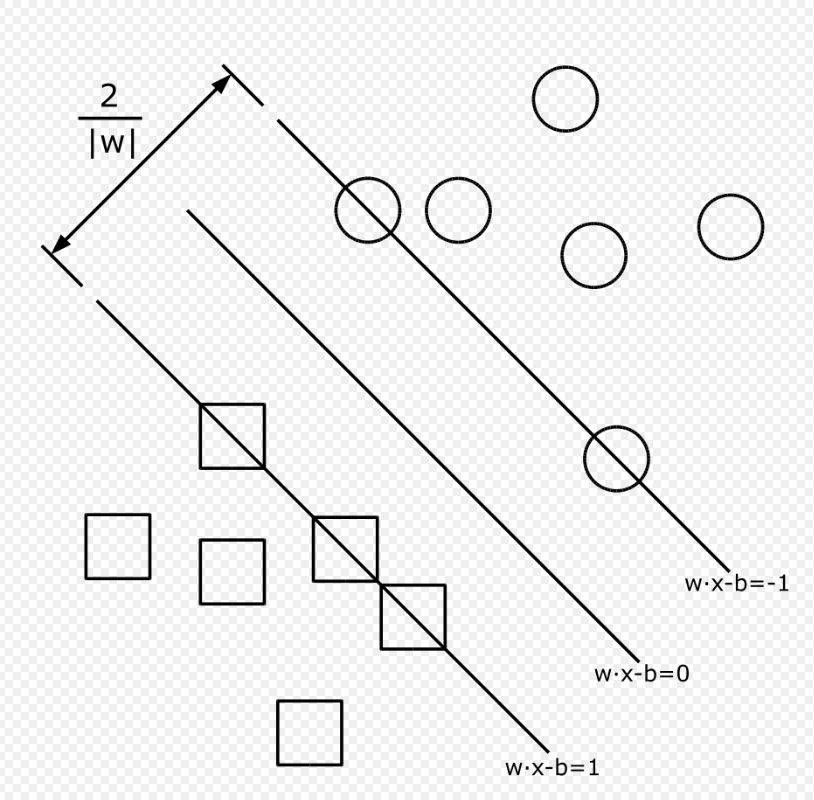
\includegraphics[width=0.5\linewidth,height=0.5\linewidth]{pictures/screenshot021}
	\caption{SVM гиперплоскость}
	\label{fig:screenshot021}
\end{figure}

Для полного разделения классов необходимо чтобы для всех i $\in [1, n]$ были выполнены неравенства:
\begin{equation}
\begin{cases}
wx_i - b \ge 1, c_i == 1 \\
wx_i - b \le -1, c_i == -1
\end{cases}
\label{eq:ref1}
\end{equation}

Тогда для того, чтобы найти оптимальную гиперплоскость нужно минимизировать $||w||$, при условиях \ref{eq:ref1}, что соотвествует такой задаче минимизации:
\begin{equation}
\begin{cases}
||w||^2 -> \min \\
c_i(wx_i - b) \ge 1, i \in [1, n]
\end{cases}
\label{eq:ref2}
\end{equation}

В случае, если классы не разделимы линейно, вводится дополнительный параметр $\epsilon_i \ge 0$, характеризующий ошибку на объектах $x_i$. Таким образом, смягчим ограничение во втором уравнении системы \ref{eq:ref2} и введём штраф за ошибку C - данный параметр позволяет регулировать соотношение между максимизацией ширины разделяющей полосы и минимизацией ошибки:
\begin{equation}
\begin{cases}
\dfrac{1}{2}||w||^2 + C\sum_{i=1}^{n}\epsilon_i -> \min_{wb\epsilon_i} \\
c_i(wx_i - b) \ge 1 - \epsilon_i, i \in [1, n] \\
\epsilon_i \ge 0
\end{cases}
\label{eq:ref3}
\end{equation}

Теперь, понимая математический аппарат работы SVM рассмотрим процесс построения классификатора для поиска объекта на изображении.

Входными векторами для SVM могут выступать различные виды признаков искомого объекта. Например, гистограмма ориентированных градиентов(HOG)\cite{b:HOG}, SIFT\cite{b:SIFT}/SURF\cite{b:SURF} дескрипторы.
Таким образом для решения задачи поиска объекта с помощью SVM необходимо выполнить следующие шаги:
\begin{enumerate}
	\item Разметить некоторое количество искомых объектов на изображении. Такие объекты будем относить к первому классу.
	\item Сгенерировать(или разметить) некоторое количество отрицательных примеров, которые точно не являются искомым объектом. Такие объекты отнесем ко второму классу.
	\item Рассчитать вектор признаков по которым мы будем обучать классификатор в каждой из размеченных(сгенерированных) точках изображения.
	\item Построить разделяющую объекты разных классов гиперплоскость, используя посчитанные в предыдущем пункте вектора признаков объектов.
	\item Для нахождения объекта на входном изображении, используя технику "скользящее окно"\cite{b:window} рассчитать вектор признаков во всевозможных окнах и определить по какую сторону от гиперплоскости находится вычисленный вектор. 
	Таким образом в итоге получится некоторый набор окон, в которых был найден искомый объект:
	\begin{figure}[h!]
		\centering
		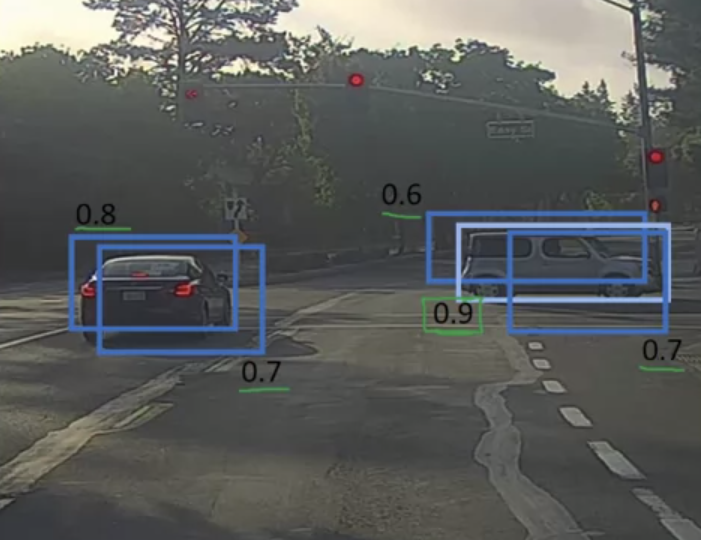
\includegraphics[width=0.7\linewidth]{pictures/screenshot024}
		\caption{Окна с объектами}
		\label{fig:screenshot024}
	\end{figure}
	\item Из найденных окон выбрать наиболее точно описывающее искомый объект. Это можно сделать выбрав окно с максимальной вероятностью нахождения искомого объекта. Например, на рисунке \ref{fig:screenshot024} для правой машины это будет окно с вероятностью 0,9.
\end{enumerate}

\subsubsection{Haar classifier}
Одним из методов поиска рельсов на изображении также может быть обучение классификатора на основе признаков Хаара. Можно заметить, что область изображения, в которой находится рельс, явно выделяется на фоне окрестностей справа и слева от рельса:
\begin{figure}[h!]
	\centering
	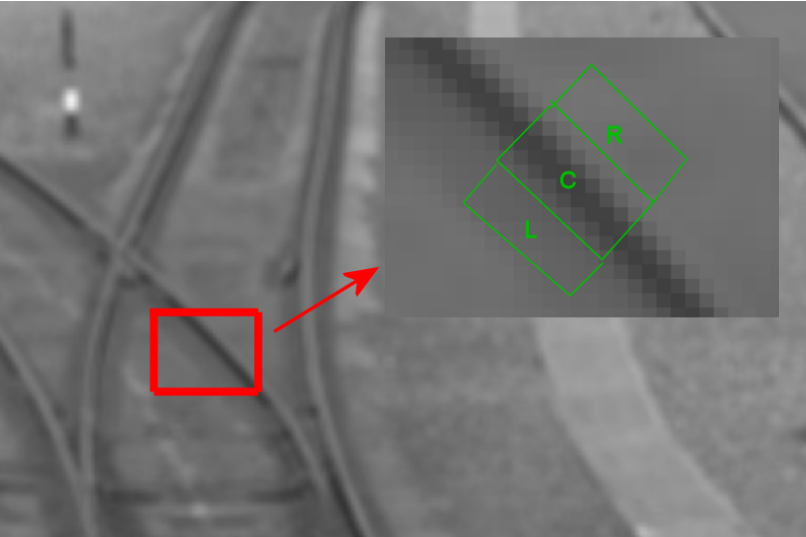
\includegraphics[width=0.7\linewidth]{pictures/screenshot23237}
	\caption{}
	\label{fig:screenshot23237}
\end{figure}\newline
Таким образом, с использованием большого датасета размеченных рельсов\cite{b:rail_scene} можно обучить классификатор, который по разности интенсивностей пикселей в черной и белой областях(рис.\ref{fig:screenshot23236}) смог бы предсказать, является выделенная область рельсом или нет. Причем рельсы могут идти под наклоном и тогда только вертикальные признаки Хаара не подойдут, поэтому нужно использовать наклонные признаки Хаара:
\begin{figure}[h!]
	\centering
	
\includegraphics[width=0.7\linewidth]{pictures/screenshot23236}
	\caption{Наклонные признаки Хаара}
	\label{fig:screenshot23236}
\end{figure}
 

\chapter{Основная часть}
\section{Метод основанный на преобразовании Хафа}
\label{houghAlgo}
\subsection{Поиск границ на изображении}
Первым шагом метода является поиск границ на входном изображении. Это делается с помощью алгоритма Canny \cite{b:canny}:
\begin{figure}[!h]
	\centering
	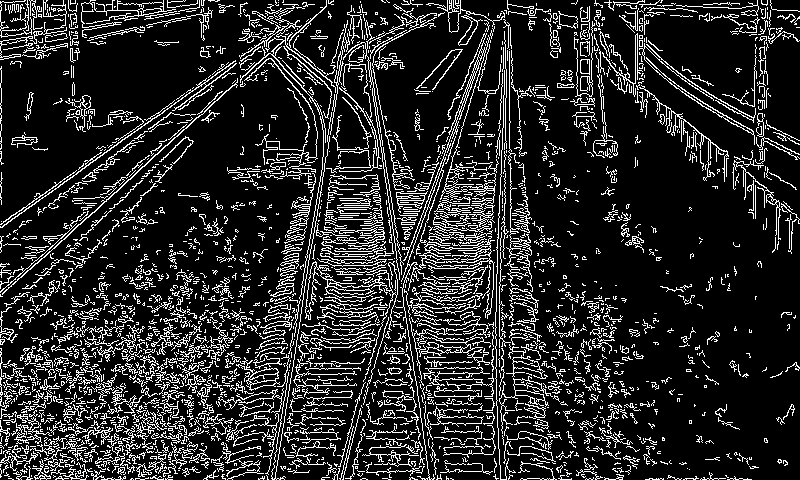
\includegraphics[width=0.9\textwidth]{pictures/canny_res}
	\caption[Применение алгоритма Canny]{Применение алгоритма Canny}
	\label{fig:cannyres}
\end{figure}

\subsection{Разбиение изображения на горизонтальные блоки}
Разбиваем изображение на горизонтальные блоки \ref{fig:horizontal_blocks}. Размер блоков уменьшается в зависимости от координаты Y на изображении, это сделано для учета перспективной проекции объектов из реального мира на изображении - чем дальше объект, тем меньше он на изображении. В идеале размер блока должен меняться по закону, показанному зеленой линией, но мы не знаем параметры камеры и поэтому используем простейшую линейную интерполяцию(y - координата на изображении отсчитывая от нижней точки, h - высота блока):
\begin{figure}[!h]
	\centering
	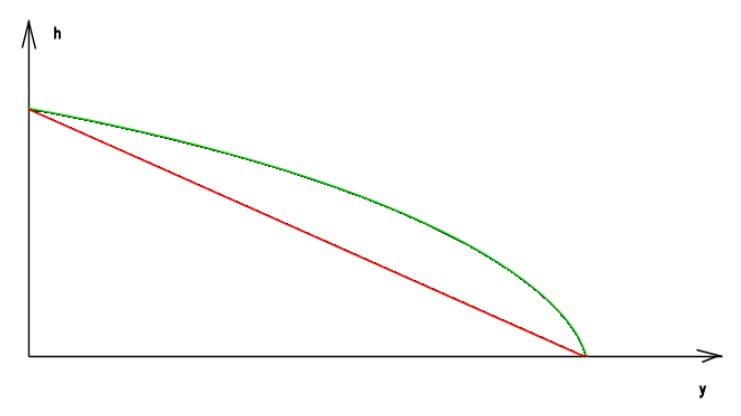
\includegraphics[width=0.6\textwidth]{pictures/graph.jpg}
	\caption[Применение алгоритма Canny]{Размер горизонтального блока}
	\label{fig:hor_block}
\end{figure}
\newpage
Формула для расчёта размера блока в зависимости от координаты y:
\newline
$blockSize = minBlockSize + \dfrac{maxBlockSize - minBlockSize}{imageHeight - maxBlockSize}y$, где  minBlockSize = 7pix, maxBlockSize = 45pix. Данные значения были выбраны из соображений минимизации процента ошибочных предсказаний стрелок и максимизации процента предсказания реальных стрелок.
В идеале размер горизонтального блока нужно рассчитывать с использованием правил перспективного проецирования\cite{b:projection}, но для этого необходимо знать параметры камеры(угол наклона, расстояния до земли).
В нашем случае эти параметры не известны, поэтому blockSize рассчитывается просто с помощью линейной интерполяции в зависимости от координаты Y.

\begin{figure}[!h]
	\centering
	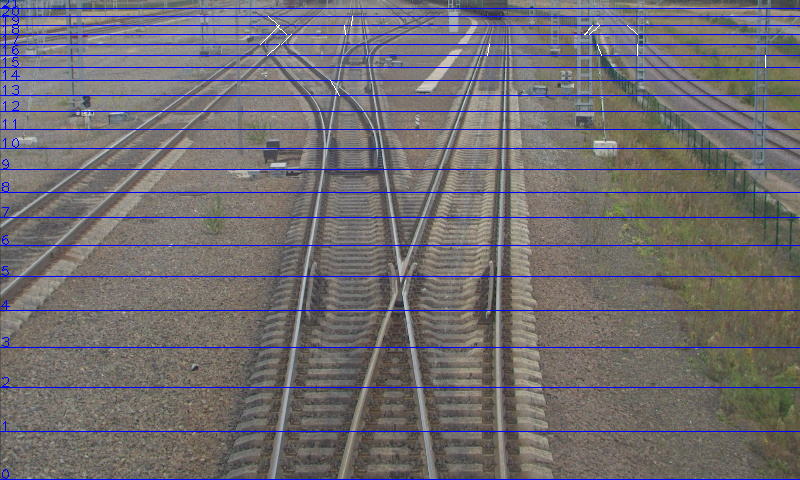
\includegraphics[width=0.9\textwidth]{pictures/horizontal_blocks.png}
	\caption[Разбиение на горизонтальные блоки]{Горизонтальные блоки}
	\label{fig:horizontal_blocks}
\end{figure}

\subsection{Поиск рельсов}\label{rails_find}
Теперь рассмотрим процесс поиска рельсов на изображении, полученном после применения алгоритма Canny\ref{fig:cannyres}.

После разбиения \ref{fig:horizontal_blocks} в каждом из горизонтальных блоков ищутся прямые линии с помощью алгоритма Хафа \cite{b:hough_transform}. Можно заметить, что прямые близкие к горизонтальным можно отсекать, т.к. они не могут относиться к рельсам. Таким образом, будем искать прямые с помощью модифицированной алгоритма Хафа, в котором $\theta \in [0;\dfrac{\pi}{3}] \cup [\dfrac{2\pi}{3};\pi]$. В качестве порогового значения аккумулятора будем использовать: $\dfrac{2\cdot blockSize}{3}$, это нужно для отсечения маленьких прямых.

Результат применения алгоритма(красным выделены найденные прямые линии в каждом блоке):
\begin{figure}[!h]
	\centering
	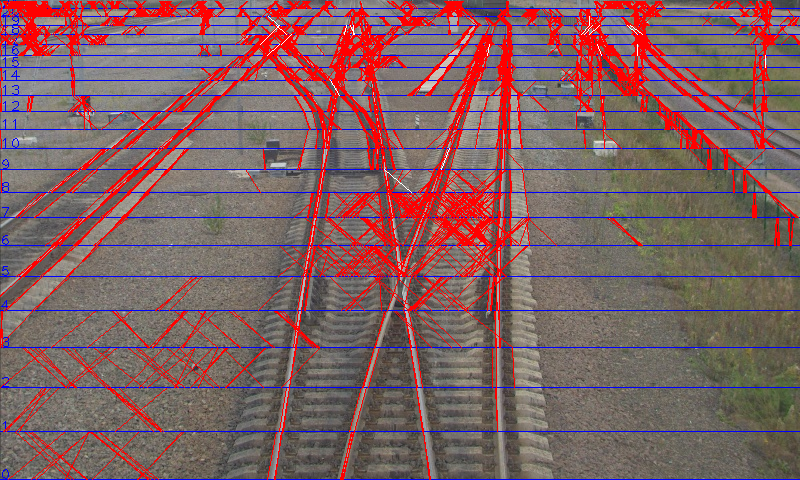
\includegraphics[width=0.9\textwidth]{pictures/hough_lines_res}
	\caption[Результат применения алгоритма]{Найденные прямые}
	\label{fig:houghlinesres}
\end{figure}

\newpage
Можно заметить много прямых образованных на шпалах(между рельсами). Это связано с тем, что на шпалах находится много граничных точек\ref{fig:cannyres}. 
Чтобы минимизировать влияние таких прямых произведем простое удаление горизонтальных рёбер: из изображения, полученного с помощью преобразования Canny удалим такие горизонтальные участки, на которых ребро встречается 3 и более пикселей подряд.
В результате получим такую картинку ребер на изображении:
\begin{figure}[!h]
	\centering
	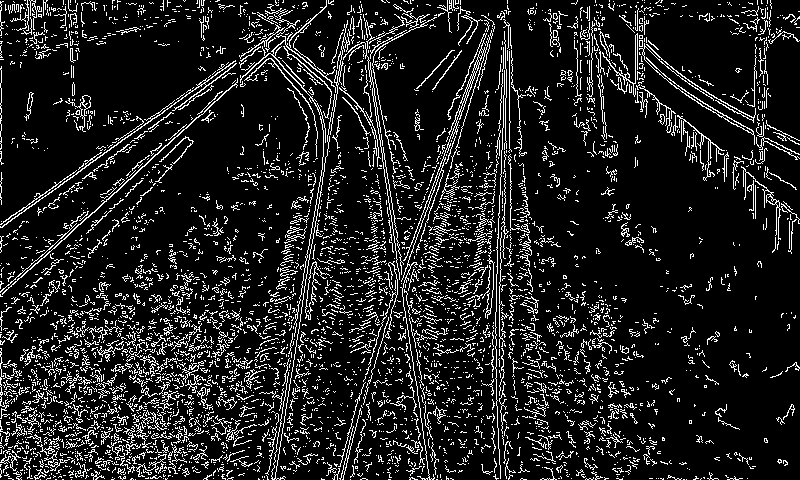
\includegraphics[width=0.9\linewidth]{pictures/screenshot0014}
	\caption{Удаление горизонтальных ребер}
	\label{fig:canny_remove_horizontal}
\end{figure}

Также видно, что от одного рельса может появляться сразу несколько прямых. Чтобы этого избежать применим аппроксимацию близких прямых одной средней прямой(координаты такой прямой будут считаться, как центр масс всех близких прямых). 
Прямые будут считаться близкими, если расстояние между верхними и нижними точками соответствующих прямых меньше заданного: \newline
$LinesEps = minLinesEps + \dfrac{maxLinesEps - minLinesEps}{imageHeight - maxLinesEps}y$, \newline 
где minLinesEps = 10 и maxLinesEps = 20 - значения полученные с учетом подсчета средней ширины рельса на изображении в зависимости от координаты Y.

Тогда после описанных выше преобразований получим следующий результат:
\begin{figure}[!h]
	\centering
	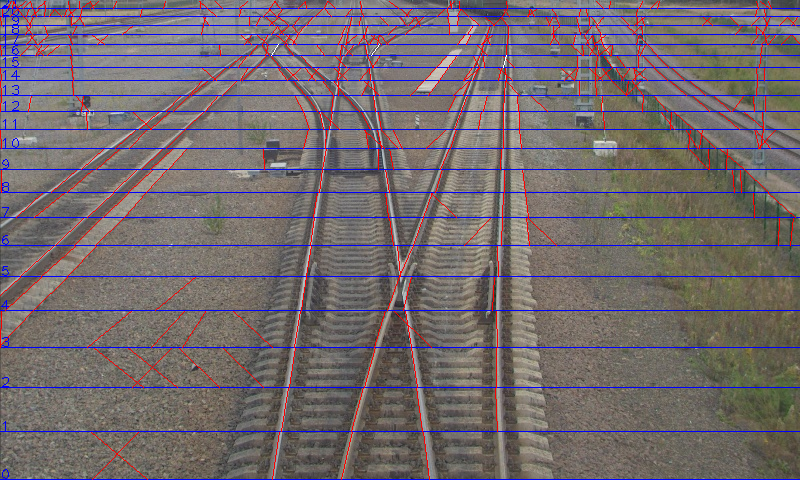
\includegraphics[width=0.9\linewidth]{pictures/screenshot0013}
	\caption{Результат поиска рельсов}
	\label{fig:screenshot0013}
\end{figure}

\subsection{Поиск стрелок}
\subsubsection{Построение графа прямых}
\label{line_graph}

Построим граф, вершинами которого будут найденные прямые. Каждая вершина будет иметь структуру: 

$(p1, p2, high_neighs, low_neighs)$, где $p1$ - нижняя точка прямой, $p2$ - верхняя точка прямой, $high_neighs$ - верхние соседи(прямые, которые выходят из прямой, соответствующей текущей вершине), $low_neighs$ - нижние соседи(прямые, которые входят в прямую, соответствующую текущей вершине). 

Ребра в графе будут строиться по следующему принципу: начиная с нижнего горизонтального блока, для каждой прямой(curLine) ищем верхних соседей в следующем блоке. Прямая(nextLine) будет считать верхним соседом, если:

$|nextLine.p1.x - curLine.p2.x| < LinesEps$, 
где LinesEps - считается также как в параграфе \ref{rails_find}.

Найденные вершины добавляются, как верхние соседи, в текущую вершину. А также текущая вершина добавляется, как нижний сосед, в каждого из верхних соседей.

Например, на рисунке \ref{fig:neighscheck}:
\begin{enumerate}
	\item прямые 1, 2 являются верхними соседями для прямой 4. А прямая 4 является нижним соседом для прямых 1 и 2.
	\item Прямая 3 лежит дальше, чем blockEps от прямой 4, поэтому между ними нет связи в графе.
	\item прямая 4 является верхним соседом для прямых 5 и 6, но не является верхним соседом для прямой 7. А прямые 5 и 6 в свою очередь являются нижними соседями для прямой 4.
\end{enumerate}
\begin{figure}[!h]
	\centering
	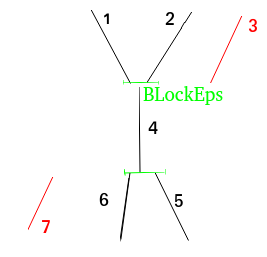
\includegraphics[width=0.7\textwidth]{pictures/neighs_check}
	\caption[Создание ребер]{Создание ребер}
	\label{fig:neighscheck}
\end{figure}
\newpage
\subsubsection{Поиск стрелок в графе}

В этом параграфе будет рассмотрен алгоритм поиска стрелок в построенном на предыдущем шаге графе. 

Алгоритм поиска пересекающихся вершин в графе: \newline
В цикле для каждой вершины графа производим следующие действия:
\begin{enumerate}
	\item Если вершина не имеет параллельного нижнего соседа - переходим к следующей вершине
	\item Для каждой пары верхних соседей текущей вершины проверяем, пересекаются ли они(\ref{intersection}), если да - верхнюю точку текущей вершины добавляем в итоговый результат найденных стрелок. Таким образом, будут найдены \nameref{fig:ycross} и \nameref{fig:xcross} пересечения.
	\begin{figure}[!h]
		\centering
		\begin{minipage}{0.45\textwidth}
			\centering
			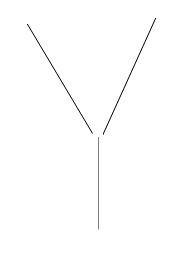
\includegraphics[width=0.7\linewidth,height=0.7\linewidth]{pictures/Y_cross}
			\caption[Y]{Y - образное}
			\label{fig:ycross}
		\end{minipage}
		\begin{minipage}{0.45\textwidth}
			\centering
			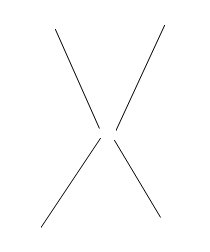
\includegraphics[width=0.7\linewidth,height=0.7\linewidth]{pictures/X_cross}
			\caption[X]{Х - образное}
			\label{fig:xcross}
		\end{minipage}
	\end{figure}
	
	\item Пункт 2) повторяется для нижних соседей текущей вершины. Таким образом, будут найдены \nameref{fig:ycrossrevert} и \nameref{fig:xcross_revert} образные пересечения.
	\begin{figure}[!h]
		\centering
		\begin{minipage}{0.45\textwidth}
			\centering
			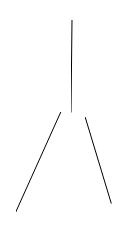
\includegraphics[width=0.7\linewidth,height=0.7\linewidth]{pictures/Y_cross_revert}
			\caption[Y - обратное]{Y - обратное}
			\label{fig:ycrossrevert}
		\end{minipage}
		\begin{minipage}{0.45\textwidth}
			\centering
			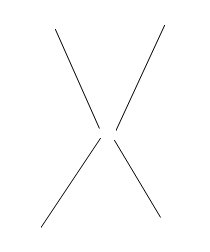
\includegraphics[width=0.7\linewidth,height=0.7\linewidth]{pictures/X_cross}
			\caption[X]{X - образное}
			\label{fig:xcross_revert}
		\end{minipage}
	\end{figure}
\end{enumerate}
\newpage

\subsubsection{Алгоритм проверки параллельности прямых}
Рассмотрим функцию проверки параллельности прямых:
\begin{enumerate}
	\item Вычисляем косинусы между прямыми и осью абсцисс.
	\begin{lstlisting}
	Ox = (1, 0)
	cos1 = cos(line1, Ox)
	cos2 = cos(line2, Ox)
	\end{lstlisting}
	\item Вычисляем разность косинусов
	\begin{lstlisting}
	cos_diff = abs(cos1, cos2)
	\end{lstlisting}
	\item Вычисляем насколько близко должны быть прямые, чтобы считать их параллельными. Тут в очередной раз применяется линейная интерполяция. Так как чем ближе рельсы к камере, тем меньше угол должен быть между ними, чтобы посчитать их параллельными. Параметры max\_parallel\_cos и min\_paralle\_cos были получены экспериментально, рассматривая результаты работы алгоритма для крайних случаев 
	реальных параллельных прямых на разных уровнях высоты.
	\begin{lstlisting}
	max_parallel_cos = 0.4
	min_paralle_cos = 0.05
	parallel_cos_eps = max_parallel_cos - (max_parallel_cos - 
	min_paralle_cos) / image_height * current_y
	\end{lstlisting}
	\item Если разность косинусов, вычисленная ранее, меньше parallel\_cos\_eps, прямые считаются параллельными.
	\begin{lstlisting}
	return cos_diff < parallel_cos_eps
	\end{lstlisting}
\end{enumerate}              
\subsubsection{Алгоритм проверки пересечения вершин}
\label{intersection}
На вход поступают v1, v2 -вершины, для которых нужно определить пересекаются ли они.
А также параметры: глубина проверки пересечений(intersection\_depth) и глубина проверки соседей(check\_neighs\_depth).
\newline
Алгоритм:
\begin{enumerate}
	\item Если глубина проверки пересечений достигла 0 - возвращаем True - вершины пересекаются.
	\begin{lstlisting}
	if intersection_depth == 0:
	return True
	\end{lstlisting}
	\item Если прямые, соответствующие вершинам НЕ параллельны - выбираем у каждой прямой параллельного верхнего соседа. Если параллельные соседи существуют, рекурсивно вызываем функцию is\_intersection с уменьшенной на единицу глубиной поиска пересечений.
	\begin{lstlisting}
	if not is_parallel(v1, v2):
	parallel_1 = v1.getParallelNeigh()
	parallel_2 = v2.getParallelNeigh()
	if parallel_1 and parallel_2:
	return is_intersection(parallel_1, parallel_2,
	intersection_depth - 1, check_neighs_depth)
	\end{lstlisting}
	\item Если глубина проверки соседей ещё не достигла нуля И у текущих вершин v1, v2 существуют параллельные им верхние соседи, то рекурсивно вызываем is\_intersection для найденных параллельных верхних соседей с уменьшенной на единицу глубиной проверки соседей.
	\begin{lstlisting}
	if check_neighs_depth > 0:
	parallel_1 = v1.getParallelNeigh()
	parallel_2 = v2.getParallelNeigh()
	if parallel_1 and parallel_2:
	return is_intersection(parallel_1, parallel_2,
	intersection_depth, check_neighs_depth - 1)
	\end{lstlisting}
	\item Если не было выполнено ни одно из первых трех условий - вершины не являются пересекающимися - вернем False.
\end{enumerate}
Описанный выше алгоритм применяется как для проверки пересечения между верхними соседями, так и между нижними соседями. 

Рассмотрим алгоритм на примере(синими линями изображены границы горизонтальных блоков): 
\newline
В данном примере рассматривается прямая 1. \newline На вход функции is\_intersection поступают соседние прямые 2 и 3, и параметры intersection\_depth = 2, check\_neighs\_depth = 1.
\newline
Если прямые 2 и 3 НЕ параллельны, то запускаем is\_intersection для прямых 4 и 5 и intersection\_depth = 1, check\_neighs\_depth = 1.
\newline
Если прямые 4 и 5 НЕ параллельны, то запускаем  is\_intersection для прямых 6 и 7 и intersection\_depth = 0, check\_neighs\_depth = 1. Теперь функция возвращает True и верхняя точка прямой 1 добавляется, как стрелка в результат.
\begin{figure}[!h]
	\centering
	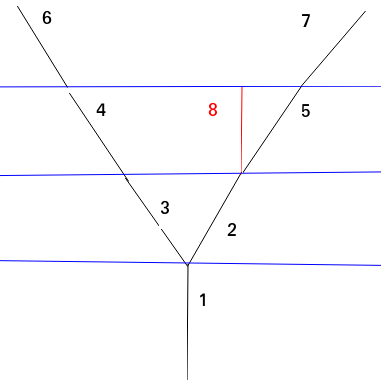
\includegraphics[width=0.7\linewidth]{pictures/intersection_example}
	\caption[Intersection]{Пример}
	\label{fig:intersectionexample}
\end{figure}

В случае пересечений между нижними соседями пример будет зеркально отражен по оси Y.

\newpage
Параметр check\_neighs\_depth нужен в случае, когда сами соседи являются параллельными(прямые 2 и 3), но их продолжения(прямые 4 и 5) уже НЕ являются параллельными. Такая ситуация характерна для Y пересечений, которые находятся близко к камере.
\begin{figure}[!h]
	\centering
	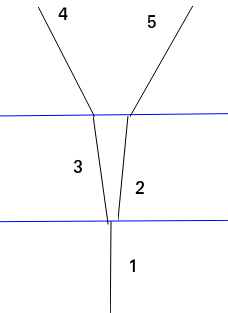
\includegraphics[width=0.3\textwidth, height=0.2\textheight]{pictures/intersection_example1}
	\caption{Рекурсивная проверка соседей}
	\label{fig:intersectionexample1}
\end{figure}

\subsubsection{Аппроксимация близких вершин}
\phantomsection
\label{approxi}
На последнем этапе близкие по расстоянию стрелки аппроксимируются их центрами масс.
Эта процедура повторяется рекурсивно, пока в результирующем массиве все стрелки не станут полностью отделимыми друг от друга.

\subsection{Сложность алгоритма}
1. Применение алгоритма Canny: O($H*W*\log(H*W)$)

2. Поиск прямых в каждом горизонтальном блоке: O($blocksCount * houghComplexity$) = O($blocksCount * edgePointsCount^{m-2}$, где m - количество параметров перебора(в нашем случае только угол, т.е. m = 1). Тогда итоговая сложность операции поиска прямых = O($blocksCount * edgePointsCount$)\newline

3. Построение графа соседей и поиск пересекающихся соседей: O($blocksCount * linesPerBlock^2$).

Итоговая сложность алгоритма: O($H*W*\log(H*W)$) + O($blocksCount * edgePointsCount$) + O($blocksCount * linesPerBlock^2$). Таким образом, видно, что в алгоритме нет дорогих по времени операций и поэтому он работает очень быстро. Время работы приведено в таблице \ref{Tab:res_hough}.


\section{Метод с построением SVM-классификатора}
\label{SVMClassifier}
Широко известна техника поиска объектов на изображении с использованием обученного SVM\cite{b:SVM} - классификатора. Применим данный подход, используя в качестве входных векторов - гистограмму ориентированных градиентов\cite{b:HOG} в окрестности размеченных стрелок. 
\subsection{Разметка изображений}
Для обучения классификатора необходимо подготовить входной датасет, который должен включать в себя различные виды стрелок(близкие/дальние Х-образные, близкие/дальние Y-образные):
\begin{figure}[!h]
	\centering
	\begin{minipage}{0.3\textwidth}
		\centering
		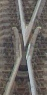
\includegraphics[width=0.3\linewidth]{pictures/screenshot3}
		\caption[X]{Х - образная стрелка}
		\label{fig:x}
	\end{minipage}
	\begin{minipage}{0.3\textwidth}
		\centering
		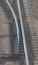
\includegraphics[width=0.3\linewidth]{pictures/screenshot4}
		\caption[Y]{Y - образная стрелка}
		\label{fig:y}
	\end{minipage}
\end{figure}

\newpage
Разметка датасета проводилась с помощью утилиты supervisely.
Видно, что изображения Х-образных стрелок сильно отличается от Y-образных стрелок. Поэтому во время разметки датасета для каждой стрелки указывался её тип(X/Y-образная). Также на первом этапе "отрицательные" примеры, которые тоже необходимы для обучения SVM тоже размечались вручную. Пример разметки изображения(зеленым показаны положительные пример, красным - отрицательные):
\begin{figure}[h!]
	\centering
	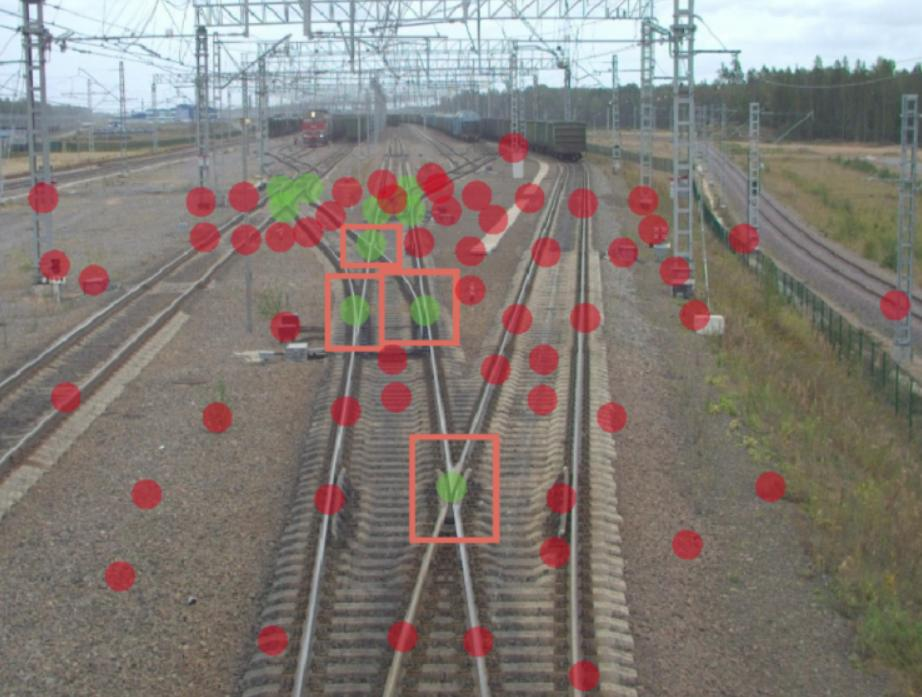
\includegraphics[width=1\linewidth]{pictures/screenshot2}
	\caption{Разметка}
	\label{fig:screenshot2}
\end{figure}

\subsection{Обучение классификатора}
Как было сказано ранее, X и Y образные стрелки сильно отличаются друг от друга. Поэтому было решено делать отдельные классификатора для разных видов стрелок. Также можно заметить, что изображения стрелок вблизи камеры и вдали от камеры отличаются(за счет более детализированной картины близи поезда):
\begin{figure}[!h]
	\centering
	\begin{minipage}{0.3\textwidth}
		\centering
		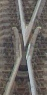
\includegraphics[width=0.3\linewidth]{pictures/screenshot3}
		\caption[X]{Стрелка вблизи камеры}
		\label{fig:x}
	\end{minipage}
	\begin{minipage}{0.3\textwidth}
		\centering
		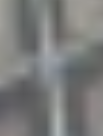
\includegraphics[width=0.3\linewidth]{pictures/screenshot5}
		\caption[Y]{Стрелка вдали от камеры}
		\label{fig:y}
	\end{minipage}
\end{figure}

Поэтому были выбраны два размера окна(большое - 48x80pix, маленькое - 12x16pix), и в зависимости от координаты Y размеченной стрелки, окно для подсчета гистограммы ориентированных градиентов данной стрелки масштабировалось к размеру большого либо маленького окна. Если $y > \dfrac{1}{5}imageHeight$, то окно масштабировалось к большему окну, иначе к меньшему. Причём  размер окна до масштабирования линейно зависит от координаты y:
\newline
\begin{equation}
\begin{cases}
winH = minWinH + \dfrac{maxWinH - minWinH}{imageHeight - maxWinH}y\\
winW = 0.7WinH\\
\end{cases}
\label{eq:windows}
\end{equation}

Таким образом, обучались по 2 классификатора(X/Y - образные стрелки) для каждого из двух размеров окна. В итоге были обучены 4 SVM - классификатора: X\_big, X\_small, Y\_big, Y\_small.

\subsection{Предсказание результаты на входном изображении}
Поиск стрелок на входном изображении происходил по следующему алгоритму:

\lstinputlisting{code.txt}

\begin{enumerate}
	\item Начиная с точки с координатой (0.7minWinH, minWinH) вычислялся текущий размер окна\ref{eq:windows} в зависимости от координаты Y, и вычислялся признак HOG в текущем окне. 
	\item После вычисления признака определялось по какую сторону от гиперплоскости, полученной в итоге обучения SVM, лежит значение признака в данной точке и принималось решение можно ли считать данную точку стрелкой.
	\item Далее окно перемещается на текущий шаг - curWinStep.
	\item Алгоритм повторяется для всех точек (x, y) с шагом curStep.
\end{enumerate}

\subsection{Первый этап обучения}
На первом этапе положительные и отрицательные примеры были размечены вручную и параметры датасета была следующие:
\begin{table}[h!]
	\begin{tabular}{|l|l|}
		\hline
		\textbf{Object}    & \textbf{Count} \\ \hline
		Y\_small        & 90             \\ \hline
		Y\_big          & 130            \\ \hline
		X\_small        & 61             \\ \hline
		X\_big          & 89             \\ \hline
		Negative\_small & 224            \\ \hline
		Negative\_big   & 394            \\ \hline
	\end{tabular}
	\label{tab:params1}
	\caption{Параметры датасета}
\end{table}
\newline
В результате получалось слишком много False Positive предсказаний классификатора на дальних стрелках:
\begin{figure}[h!]
	\centering
	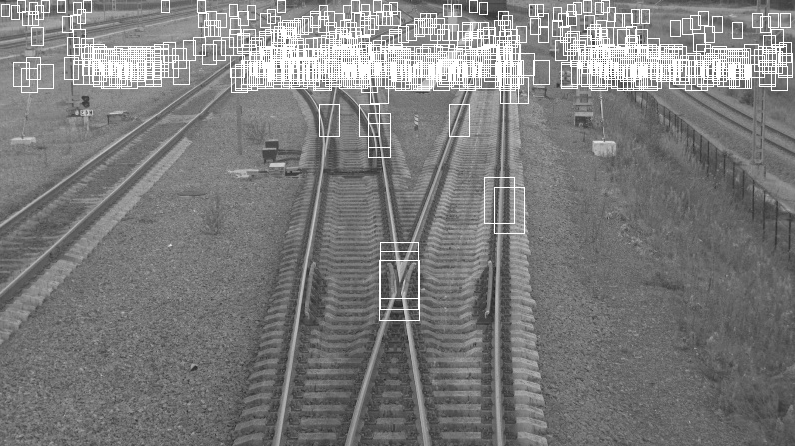
\includegraphics[width=0.7\linewidth]{pictures/screenshot32}
	\caption{Плохой результат}
	\label{fig:screenshot32}
\end{figure}

\subsection{Второй этап обучения}
Следующим этапом было уменьшение False Positive предсказаний за счет увеличения негативных примеров в обучающей выборке. На этот раз негативные примеры генерировались автоматически на каждом из изображений обучающей выборке. Генерация происходила в виде сетки(для верхней части изображения шаг генерации меньше, так как именно там было зафиксировано очень много False Positive предсказаний):
\begin{figure}[h!]
	\centering
	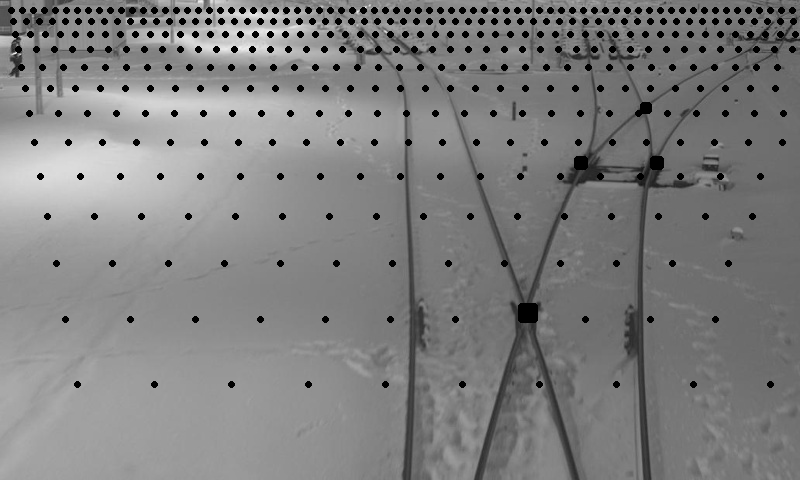
\includegraphics[width=0.7\linewidth]{pictures/grid_negative.png}
	\caption{Разметка}
	\label{fig:screenshot32}
\end{figure}
\newline
Также в связи с увеличением кол-ва негативных примеров нужно увеличить кол-во позитивных примеров. Для каждого позитивного примера все точки в некоторой его окрестности тоже добавлялись в обучающую выборку(размер окрестности линейно зависит от координаты Y стрелки):
\begin{figure}[!h]
	\centering
	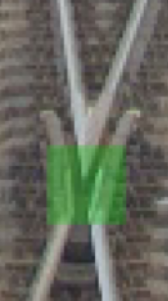
\includegraphics[width=0.1\linewidth]{pictures/screenshot2323}
	\caption{Разметка}
	\label{fig:screenshot2323}
\end{figure}
\newpage
Параметры датасета получились следующие:
\begin{table}[!h]
	\begin{tabular}{|l|l|}
		\hline
		\textbf{Object} & \textbf{Count} \\ \hline
		Y\_small        & 856            \\ \hline
		Y\_big          & 2724           \\ \hline
		X\_small        & 384            \\ \hline
		X\_big          & 1972           \\ \hline
		Negative\_small & 75500          \\ \hline
		Negative\_big   & 146200         \\ \hline
	\end{tabular}
	\label{tab:params2}
	\caption{Параметры датасета}
\end{table}

Результат работы классификатора:
\begin{figure}[!h]
	\centering
	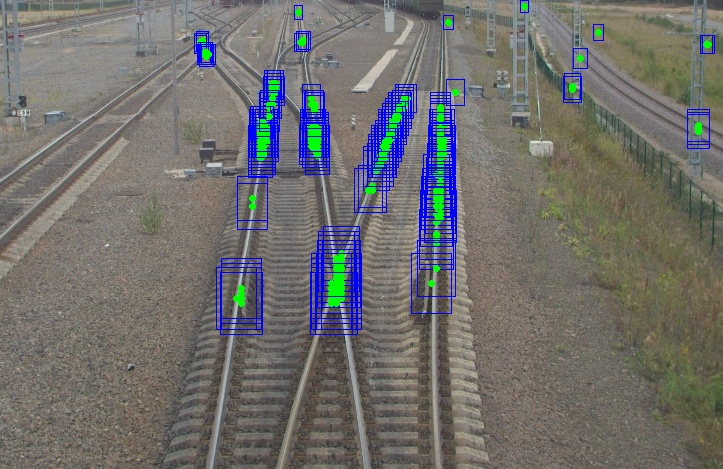
\includegraphics[width=0.7\linewidth]{pictures/screenshot2324}
	\caption{Результата классификатора}
	\label{fig:screenshot2324}
\end{figure}

\subsection{Третий этап обучения}
На предыдущем этапе мы избавились от большего числа False Positive предсказаний в дальней части изображения, но при этом теперь рельсы плохо отличаются от стрелок в ближней части изображения. 
Чтобы этого избежать было решено добавить в обучающую выборку точки, принадлежащие рельсам(но НЕ принадлежащие стрелкам), как негативные примеры. Для этого был разработан алгоритм поиска рельсов на основе метода предложенного в статье\cite{b:growing_up}. Краткий обзор этой статьи приведен выше в главе \ref{obzor}. Результат работы алгоритма поиска рельсов следующий:
\begin{figure}[h!]
	\centering
	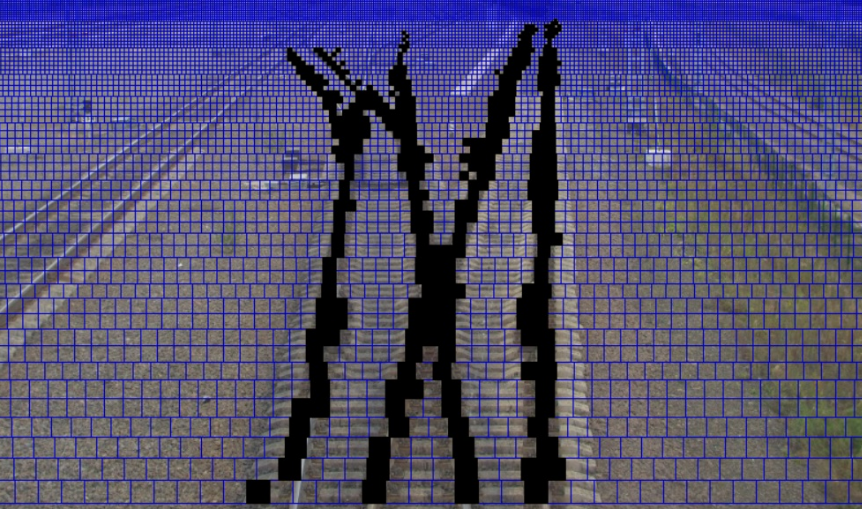
\includegraphics[width=0.7\linewidth]{pictures/screenshot2325}
	\caption{Поиск рельсов}
	\label{fig:screenshot2325}
\end{figure}
\newpage
Применив данный алгоритм ко всем изображениям из обучающей выборки, и добавив к негативным примерам полученные рельсы получаем следующую картинку разметки каждого изображения:
\begin{figure}[h!]
	\centering
	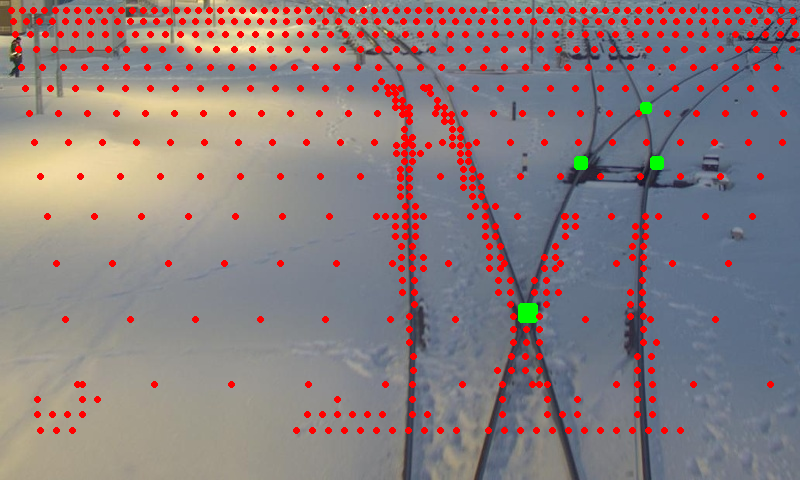
\includegraphics[width=0.7\linewidth]{pictures/full_dataset}
	\caption{Полная разметка}
	\label{fig:screenshot2325}
\end{figure}

Параметры обучающего датасета:
\begin{table}[!h]
	\begin{tabular}{|l|l|}
		\hline
		\textbf{Object} & \textbf{Count} \\ \hline
		Y\_small        & 4106           \\ \hline
		Y\_big          & 20258          \\ \hline
		X\_small        & 2260           \\ \hline
		X\_big          & 12320          \\ \hline
		Negative\_small & 132888         \\ \hline
		Negative\_big   & 133350         \\ \hline
	\end{tabular}
	\label{tab:params3}
	\caption{Параметры датасета}
\end{table}

Результаты предсказания:
\begin{figure}[!h]
	\centering
	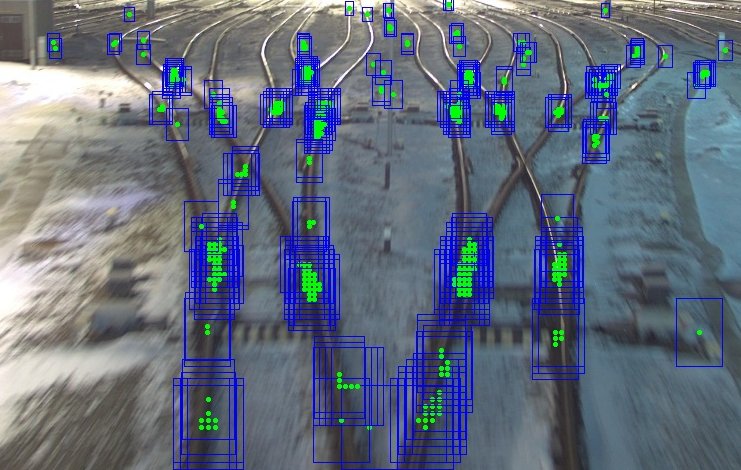
\includegraphics[width=0.8\linewidth]{pictures/screenshot2326}
	\caption{Пример результата 1}
	\label{fig:screenshot2326}
\end{figure}
\begin{figure}[h!]
	\centering
	\includegraphics[width=0.8\linewidth]{pictures/screenshot2327}
	\caption{Пример результата 2}
	\label{fig:screenshot2327}
\end{figure}\newpage
\subsection{Подтверждение стрелок}
\label{crossDetection}
Видно, что теперь в большинстве случаев именно в окрестности стрелок высокая концентрация позитивных предсказаний. Теперь предстоит решить задачу выбора таких мест концентрации позитивных предсказаний, в которых действительно находится стрелка. 

Рассмотри следующий алгоритм для подтверждения стрелок:

Для каждого изображения из тестовой выборки запускаем алгоритм предсказания стрелок. На каждом из изображений известны ожидаемые положения стрелок. Можно рассчитать, сколько в среднем приходится предсказаний на одну ожидаемую стрелку(сколько предсказанных стрелок находятся в некоторой окрестности ожидаемой стрелки). После применения такой процедуры к каждой ожидаемой стрелке, получим среднее число предсказнных стрелок приходящихся на одну ожидаемую стрелку. Назовем это число packageNumber.

Теперь можно применить уже описанный ранее алгоритм кластеризации близких предсказанных стрелок\ref{approxi}. Но уже с подсчетом кол-ва стрелок, которые аппроксимируют одну итоговую стрелку. После чего необходимо отсечь те итоговые стрелки, которые аппроксимируют меньше чем packageNumber предсказанных стрелок. На рисунке ниже зеленым выделены все предсказнные стрелки, а красным - итоговые стрелки, полученные после аппроксимации и отсечения по порогу:
\begin{figure}[h!]
	\centering
	\includegraphics[width=0.7\linewidth]{pictures/package1}
	\caption{Аппроксимация центрами масс}
	\label{fig:package1}
\end{figure}
\newpage
Также для аппроксимации групп близко расположенных стрелок и отсечения выбросов был использован известный алгоритм кластеризации DBSCAN\cite{b:dbscan}. 
\begin{figure}[h!]
	\centering
	\includegraphics[width=0.7\linewidth]{pictures/dbscan}
	\caption{DBSCAN}
	\label{fig:package1}
\end{figure}

Видно, что оба алгоритма работают приемлемо, в главе \ref{statRes} будут рассмотрены статистические результаты работы для обоих алгоритмов кластеризации.

\subsection{Сложность алгоритма}
Рассмотрим сложность работы функции предсказания обученного SVM-классификатора.

В каждом окне нужно вычислить hog=HOG() и вызвать функцию Classifier.predict(hog). Всего окон получается: 
\begin{equation}
windowsCount = \dfrac{H}{windowSize(y)} * \dfrac{W}{windowSize(y)}
\label{eq:windowCount}
\end{equation}, здесь $windowSize(y)$ - размер окна в зависимости от координаты Y на изображении.

Рассчитаем размерность вектора HOG для большого и маленького окна. Большое окно имеет размер 80x48pix. Размер блоков, на которые разбивается окно для расчёта HOG - 8х8pix. Для нормализации блоки разбиваются на группы по 2х2 блока(будет называть такие группы большими блоками).
\begin{figure}[h!]
	\centering
	\includegraphics[width=0.7\linewidth]{pictures/screenshot02332}
	\caption{}
	\label{fig:screenshot02332}
\end{figure}

Больших блоков всего будет: $(\dfrac{80}{8} - 1)* (\dfrac{48}{8} - 1) = 45$. Размерность HOG в одном маленьком блоке 8x8pix равна 9(всего 9 направлений). Таким образом в каждом большом блоке гистограмма имеет размерность: 9 * (2 * 2) = 36. Тогда размер вектора HOG для всего большого окна будет: 45 * 36 = 1620. Аналогично можно рассчитать размерность HOG для маленького окна и получить 216(в маленьком окне размерность каждого блока бралась 4x4pix).

Самая дорогая по времени операция это вычисление функции Classifier.predict(hog). Данная операция вызывается для каждого сканирующего окна(их количество описано выше \ref{eq:windowCount}). Функция предиктор в случае SVC классификатора выглядит следующим образом: $\sum_{i \in SV} y_i\alpha_i K(x_i, x) + b$, где SV - множество опорных векторов($x_i$ - i-ый опорный вектор, $y_i$ - номер класса i-го вектора, $\alpha_i$ - вес i-ого вектора), полученных в процессе обучения классификатора, K - ядерная функция(в нашем случае используется ядро Гаусса $\exp^{-\gamma*(x-x_*)^2}$). Таким образом, сложность вычисления функции Classifier.predict будет O(NumOfSV * d), где d - размерность вектора x(в нашем случае это размерность HOG), а NumOfSV - кол-во опорных векторов. 

Рассмотрим кол-во опорных векторов для нашего обученного классификатора:
\begin{enumerate}
	\item SV(Y\_big) = 10509
	\item SV(X\_big) = 5163
	\item SV(Y\_small) = 6887
	\item SV(X\_small) = 6381
\end{enumerate}
Количество 10509, 5163, 6887, 6381 объяснить аналитически нельзя, так как опорные вектора выбираются так, чтобы гиперплоскость, которая строится в процессе обучения SVM проходила максимально оптимально(решается задача оптимизации и заранее нельзя сказать сколько будет опорных векторов, это тесно связано с конкретным датасетом, с тем, как расположились обучающие вектора в пространстве).

Таким образом, видно, что количество опорных векторов и размерность вектора X для SVM-классификатора достаточно большие, что приводит к долгому времени работы алгоритма.
Для самой большой модели Y\_big необходимо выполнить 10509 * 1620 = 17 * $10^6$ операций.

По результатам тестирования среднее время работы классификатора на изображении составило: от 16 до 42 секунд. Тестирование проводилось на процессоре Intel Core i7, частота 800 MHz - 3.50 GHz на операционных системах Windows/Ubuntu.

\newpage
\chapter{Результаты}

\section{Описание данных для тестирования}
Для тестирования алгоритма было размечено 192 фотографии ж/д путей, сделанных с локомотива. Часть фотографий была сделана при дневном свете \ref{fig:res1}, а часть при искусственном \ref{fig:res3}. Также имеются изображения, сделанные в летний\ref{fig:res1} и в зимний период \ref{fig:res4}.

Параметры датасета:
\begin{enumerate}
	\item Всего стрелок размечено: 1357
	\item Среднее количество стрелок на одном изображении: 7
	\item Около 70\% изображений сделаны в летний период. Около 30\% в зимний.
\end{enumerate}

\section{Результаты работы алгоритма, основанного на преобразовании Хафа}
\subsection{Примеры работы алгоритма}
Результаты работы на изображении сделанном при дневном:
\begin{figure}[!h]
	\centering
	\includegraphics[width=0.7\linewidth]{pictures/screenshot0015}
	\caption{Пример 1}
	\label{fig:res1}
\end{figure}
\begin{figure}[!h]
	\centering
	\includegraphics[width=0.7\linewidth]{pictures/screenshot0016}
	\caption{Пример 2}
	\label{fig:res2}
\end{figure}
\newpage

Истинное положение стрелок (маркеры) на рисунках \ref{fig:res1}, \ref{fig:res2}, \ref{fig:res3}, \ref{fig:res4} - не обозначены, так как их положения очевидны

Видно, что есть большие стрелки - те, которые находятся достаточно близко к камере, алгоритм распознает очень хорошо. С маленькими стрелками есть небольшие проблемы, например на изображении \ref{fig:res2} самая дальняя маленькая стрелка слева не распозналась.\newline
Также видно, что достаточно много false positive стрелок получившихся от столбов и заборов. Один из способов их подавления - использовать алгоритм Region growing up(\cite{b:growing_up}) для сегментации изображения снизу вверх.

Теперь рассмотрим результат работы алгоритма при других погодных условиях и искусственном свете. Видно, что алгоритм хорошо справляется и с такими изображениями.
\begin{figure}[!h]
	\centering
	\includegraphics[width=0.7\linewidth]{pictures/screenshot0017}
	\caption{Искусственный свет}
	\label{fig:res3}
\end{figure}

\newpage
Теперь посмотрим на пример изображения, на котором алгоритм выдал очень плохой результат:
\begin{figure}[h!]
	\centering
	\includegraphics[width=0.7\linewidth]{pictures/screenshot0018}
	\caption{}
	\label{fig:res4}
\end{figure}
Видно, что на изображении есть ярко освещенные солнцем участки, и темная тень от поезда, в связи с этим алгоритм Отцу \cite{b:otsu} выдал достаточно высокое значение пороговых фильтров и рельсы, находящиеся в тени не были восприняты как рёбра алгоритмом Canny\cite{b:canny}. В следствии чего соответствующие рельсам линии не были найдены алгоритмом Хафа \cite{b:hough_transform}.
\begin{figure}[h!]
	\centering
	\includegraphics[width=0.7\linewidth]{pictures/screenshot0019}
	\caption{Плохое нахождение ребер}
	\label{fig:bad_canny}
\end{figure}
\begin{figure}[h!]
	\centering
	\includegraphics[width=0.7\linewidth]{pictures/screenshot0020}
	\caption{Плохое обнаружение линий}
	\label{fig:bad_lines}
\end{figure}

\newpage
\subsection{Статистические результаты}
Вспомним о том, что мы не знаем параметры камеры и поэтому ширину горизонтальных блоков выбираем с помощью линейной интерполяции \ref{line_graph}. Интерполяция происходит между значениями maxBlockSize и minBlockSize. 
Рассмотрим зависимость результатов обнаружения от выбора этих параметров(Тестирование проводилось на процессоре Intel Core i7, частота 800 MHz - 3.50 GHz.):
\begin{table}[!h]
	\caption{Результат алгоритма на основе преобразования Хафа}
	\begin{tabular}{|c|c|c|l|l|}
		\hline
		\multicolumn{1}{|l|}{\textbf{minBlockEps}} & \multicolumn{1}{l|}{\textbf{maxBlockEps}} & \multicolumn{1}{l|}{\textbf{time(s)}} & \textbf{Precision} & \textbf{Recall} \\ \hline
		7                                          & 45                                        & 0.27                                   & 0.43               & 0.76            \\ \hline
		7                                          & 30                                        & 0.03                                   & 0.34                & 0.83            \\ \hline
		20                                         & 45                                        & 0.02                                  & 0.64               & 0.3             \\ \hline
	\end{tabular}
	\label{Tab:res_hough}
\end{table}
\newline
$Precistion = \dfrac{TruePositive}{TruePositive + FalsePositive}$ - процент корректных предсказаний.
\newline
$Recall = \dfrac{TruePositive}{TruePositive + FalseNegative}$ - мера, определяющая как хорошо алгоритм находит позитивные примеры(стрелки)

Видно, что при уменьшении максимального размера блока, уменьшается процент корректных предсказаний. И увеличивается количество найденных положительных примеров. 

Также если увеливать минимальный размер блока, то растет точность, но падает процент найденных стрелок.

При большой нижней границе minBlockEps далекие стрелки вообще не находятся, зато хорошо ищутся близкие стрелки, вот пример для minBlockEps = 20pix:
\begin{figure}[!h]
	\centering
	\includegraphics[width=0.7\linewidth]{pictures/45_20.png}
	\caption[]{Большие горизонтальные блоки}
	\label{fig:45_20}
\end{figure}

\section{Результаты работы алгоритма с построением SVM-классификатор}
\subsection{Примеры работы алгоритма}
Летнее время года:
\begin{figure}[!h]
	\centering
	\includegraphics[width=0.7\linewidth]{pictures/103.png}
	\caption[Лето]{Лето}
	\label{fig:103}
\end{figure}
\newpage
Зимнее время года:
\begin{figure}[!h]
	\centering
	\includegraphics[width=0.7\linewidth]{pictures/146.png}
	\caption[Зима]{Зима}
	\label{fig:105}
\end{figure}
\newline
Искусственный свет:
\begin{figure}[!h]
	\centering
	\includegraphics[width=0.7\linewidth]{pictures/isk.png}
	\caption[Искусственное освещение]{}
	\label{fig:isk}
\end{figure}

Видно, что в целом алгоритм устойчив к различным условиям съёмки и находит большинство стрелок на изобржении. Рассмотрим подробнее статистические результаты.

\subsection{Статистические результаты}
\label{statRes}
Рассмотрим зависимость точности результата от выбора алгоритма кластеризации и параметров этого алгоритма. 

Алгоритм\ref{crossDetection} показал, что в среднем на одну ожидаемую стрелку приходится 13 предсказанных стрелок в окрестности. Но если использовать эту границу при отсечении, мы потеряем многие стрелки, которые были предсказаны меньшим числом голосов. Поэтому необходимо выбрать такую границу, при которой результат работы алгоритма был бы лучшим.
Поэтому было проведено исследование зависимости результата(Precision/Recall) от порога предсказанных в окрестности стрелок.

Результаты при применении алгоритма кластеризации основанного на аппроксимации центрами масс:
\begin{figure}[h!]
	\centering
	\includegraphics[width=0.7\linewidth]{pictures/screenshot224}
	\caption{Центры масс}
	\label{fig:screenshot224}
\end{figure}
\newpage
Результаты при применении алгоритма кластеризации DBSCAN\cite{b:dbscan}(он тоже принимает на вход минимальное кол-во точек в кластере):
\begin{figure}[h!]
	\centering
	\includegraphics[width=0.7\linewidth]{pictures/screenshot223}
	\caption{DBSCAN}
	\label{fig:screenshot223}
\end{figure}

\begin{equation}
F1 = 2 \dfrac{precision * recall}{precision + recall}
\end{equation} - среднее гармоническое между precision и recall. Эта метрика дает возможность судить о балансе между precision и recall. В лучшем случае F1 = 1 - идеальный баланс между precision и recall.

Видно, что при увеличении требуемого для подтверждения кол-ва предсказанных стрелок в окрестности(PackageNumber) растет точность предсказаний(Precision) и падает процент найденных стрелок(Recall).

Также по графику зависимости F1(PackageNumber) видно, что наибольшее значения F1 достигает при PackageNumber = 9. 
Если взять PackageNumber = 9, то получим:\newline
Precision(the percentage of predictions are correct): 0.76\newline
Recall(measures how good you find all the positives): 0.71\newline
F1(perfect precision and recall): 0.73\newline
Именно такие параметры являются лучшими с точки зрения метрики F1.

Причём видно, что оба алгоритма кластеризации дают приблизительно одинаковые результат(F1=[0.72,0.73]). 

Однако есть один существенный недостаток этого алгоритма. Если шаг, с которым окно перемещается в процессе предсказания результата очень мал, то количество необходимых вызовов функции предиктора у SVM-классификатора очень большое, что приводит к долгому времени работы.

Поэтому было решено сделать шаг скользящего окна большим и при этом уменьшить порог находящихся радом предсказанных стрелок(PackageNumber) до 2(это значение было вычислено аналогично с предыдущим исследованием, исходя из оптимального значения метрики F1). 
Таким образом, удалось уменьшить время работы в 6.5 раз и при этом не потерять и даже немного улучшить показатель метрики F1 для обоих алгоритмов кластеризации предсказанных точек.
\begin{figure}[h!]
	\centering
	\includegraphics[width=0.7\linewidth]{pictures/screenshot23238}
	\caption{Результаты для большого шага окна}
	\label{fig:screenshot23238}
\end{figure}\newline
Наилучшие показатели достигаются при PackageNumber=2:\newline
Precision: 0.65\newline
Recall: 0.86\newline
F1: 0.74


\chapter{Заключение}
В ходе работы был размечен датасет из 1357 ж/д стрелок на изображениях, сделанных с локомотива поезда в разных погодных условиях. 

Был разработан алгоритм на основе преобразования Хафа\ref{houghAlgo}, который показал достаточно большую способность к обнаружению стрелок(Recall=0.76), но при этом точность предсказаний оказалась очень низкой(Precision=0.43) из-за большего количество False Positive обнаружений, которые возникают из-за шума на изображении.

Также был обучен SVM-классификатор\ref{SVMClassifier}, который показал достаточно хорошую способность к обнаружению стрелок(Recall=0.86) и при этом хорошую точность предсказаний(Precision=0.65). 

Алгоритм на основе преобразования Хафа работает в разы быстрее алгоритма на основе SVM-классификатора, но точность предсказания у SVM-классификатора значительно выше.

Таким образом, можно сделать вывод о том, что для задачи поиска ж/д стрелок на изображении метод с обучением показал большую точность и устойчивость к шумам. В дальнейших планах попробовать использовать другие входные вектора для обучения SVM-классификатора и увеличить размер обучающего датасета для повышения вариативности исходных данных.

\newpage
%\addcontentsline{toc}{section}{Список литературы}
\begin{thebibliography}{2}
	\bibitem{b:hough_transform}
	\textbf{Преобразование Хафа}. Википедия. [Электронный ресурс] URL - 
	\href{https://en.wikipedia.org/wiki/Hough\_transform}{https://en.wikipedia.org/wiki/Hough\_transform}
	
	\bibitem{b:canny}
	\textbf{Алгоритм Canny}. [Электронный ресурс] URL - 
	\href{https://habr.com/ru/post/114589/}{https://habr.com/ru/post/114589/}
	
	\bibitem{b:otsu}
	\textbf{Алгоритм Отцу}. [Электронный ресурс] URL - 
	\href{https://docs.opencv.org/2.4/doc/tutorials/imgproc/threshold/threshold.html}{https://docs.opencv.org/2.4/doc/tutorials/imgproc/threshold/threshold.html}
	
	\bibitem{b:projection}
	\textbf{Перспективная проекция}. [Электронный ресурс] URL - 
	\href{http://stratum.ac.ru/education/textbooks/kgrafic/lection04.html}{http://stratum.ac.ru/education/textbooks/kgrafic/lection04.html}
	
	\bibitem{b:growing_up}
	\textbf{Efficient railway tracks detection and turnouts recognition method using HOG features}. [Электронный ресурс] URL - 
	\href{https://link.springer.com/article/10.1007/s00521-012-0846-0}{https://link.springer.com/article/10.1007/s00521-012-0846-0}
	
	\bibitem{b:hough_work1}
	\textbf{Vision based rail track and switch recognition for self-localization of trains in a rail network}. [Электронный ресурс] URL - 
	\href{https://ieeexplore.ieee.org/document/5940466?denied=}{https://ieeexplore.ieee.org/document/5940466?denied=}
	
	\bibitem{b:HOG}
	\textbf{Histogram of oriented gradients}. Википедия. [Электронный ресурс] URL - 
	\href{https://en.wikipedia.org/wiki/Histogram_of_oriented_gradients}{https://en.wikipedia.org/wiki/Histogram\_of\_oriented\_gradients}
	
	\bibitem{b:SIFT}
	\textbf{Scale-invariant feature transform}. [Электронный ресурс] URL - 
	\href{https://en.wikipedia.org/wiki/Scale-invariant_feature_transform}{https://en.wikipedia.org/wiki/Scale-invariant\_feature\_transform}
	
	\bibitem{b:edge_match}
	\textbf{Using Partial Edge Contour Matches for Efficient Object Category
		Localization ,Hayko Riemenschneider, Michael Donoser and Horst
		BischofProceedings of European Conference on Computer Vision}. [Электронный ресурс] URL - 
	\href{http://www.icg.tugraz.at/Members/hayko/partial-contour-efficient-
		matching}{http://www.icg.tugraz.at/Members/hayko/partial-contour-efficient-
		matching}
	
	\bibitem{b:SURF}
	\textbf{Speeded up robust features}. [Электронный ресурс] URL - 
	\href{https://en.wikipedia.org/wiki/Speeded\_up_robust\_features}{https://en.wikipedia.org/wiki/Speeded\_up\_robust\_features}
	
	\bibitem{b:SVM}
	\textbf{A Library for Support Vector Machines}. [Электронный ресурс] URL - 
	\href{https://www.csie.ntu.edu.tw/~cjlin/papers/libsvm.pdf}{https://www.csie.ntu.edu.tw/~cjlin/papers/libsvm.pdf}
	
	\bibitem{b:decision_tree}
	\textbf{Decision tree}. [Электронный ресурс] URL - 
	\href{https://en.wikipedia.org/wiki/Decision\_tree}{https://en.wikipedia.org/wiki/Decision\_tree}
	
	\bibitem{b:knn}
	\textbf{K-nearest neighbors algorithm}. [Электронный ресурс] URL - 
	\href{https://en.wikipedia.org/wiki/K-nearest\_neighbors\_algorithm}{https://en.wikipedia.org/wiki/K-nearest\_neighbors\_algorithm}
	
	\bibitem{b:window}
	\textbf{Sliding window}. [Электронный ресурс] URL - 
	\href{https://www.pyimagesearch.com/2015/03/23/sliding-windows-for-object-detection-with-python-and-opencv/}{https://www.pyimagesearch.com/2015/03/23/sliding-windows-for-object-detection-with-python-and-opencv/}
	
	\bibitem{b:lane_detection}
	\textbf{Robust lane detection and tracking for lane departure warning}. [Электронный ресурс] URL - 
	\href{https://ieeexplore.ieee.org/document/6384266}{https://ieeexplore.ieee.org/document/6384266}
	
	\bibitem{b:lane_detection_hough}
	\textbf{Double Lane Line Edge Detection Method Based on
		Constraint Conditions Hough Transform}. [Электронный ресурс] URL - 
	\href{https://ieeexplore.ieee.org/document/8572535}{https://ieeexplore.ieee.org/document/8572535}
	
	\bibitem{b:dbscan}
	\textbf{DBSCAN cluster}. [Электронный ресурс] URL - 
	\href{https://ru.wikipedia.org/wiki/DBSCAN}{https://ru.wikipedia.org/wiki/DBSCAN}
	
	\bibitem{Gonsales}
	\textbf{Цифровая обработка изображений.}
	Гонсалес Р., Вудс Р.
	Издание 3-е, исправленное и дополненное
	Москва: Техносфера, 2012. – 1104 с. 
	
	\bibitem{Gruzman}
		\textbf{Цифровая обработка изображений в информационных системах: Учебное пособие.} Грузман И.С., Киричук В.С., Косых В.П., Перетягин Г.И., Спектор А.А. - Новосибисрк: Изд-во НГТУ, 2002. - 352 c.
	
	\bibitem{Vapnik}
	\textbf{Distribution-dependent Vapnik chervonenkis
		bounds}. V. Nicolas , A. Robert, European Conference on Computational Learning Theory, pp 230-
	240, November 1999.
	
	\bibitem{b:f1}
	\textbf{F1 score}. [Электронный ресурс] URL - 
	\href{https://en.wikipedia.org/wiki/F1_score}{https://en.wikipedia.org/wiki/F1\_score}
	
	\bibitem{b:inverse_mapping}
	\textbf{A New Lane Line Segmentation and Detection Method based on Inverse
		Perspective Mapping}. [Электронный ресурс] URL - 
	\href{https://pdfs.semanticscholar.org/fb7a/76f7994cfc06783e65c58537876ee7c6af7b.pdf}{https://pdfs.semanticscholar.org/fb7a/76f7994cfc06783e65c58537876ee7c6af7b.pdf}
	
	\bibitem{b:hough_fast}
	\textbf{A FAST DECISION TECHNIQUE FOR HIERARCHICAL HOUGH
		TRANSFORM FOR LINE DETECTION}. [Электронный ресурс] URL - 
	\href{https://arxiv.org/ftp/arxiv/papers/1007/1007.0547.pdf}{https://arxiv.org/ftp/arxiv/papers/1007/1007.0547.pdf}
	
	\bibitem{b:rail_scene}
	\textbf{A dataset for rail scene understanding}. [Электронный ресурс] URL - 
	\href{http://openaccess.thecvf.com/content_CVPRW_2019/papers/Autonomous\%20Driving/Zendel_RailSem19_A_Dataset_for_Semantic_Rail_Scene_Understanding_CVPRW_2019_paper.pdf}{http://openaccess.thecvf.com/content\_CVPRW\_2019/papers/Autonomous\%20Driving/Zendel\_RailSem19\_A\_Dataset\_for\_Semantic\_Rail\_Scene\_Understanding\_CVPRW\_2019\_paper.pdf}
	
\end{thebibliography}		  		 		